\documentclass[10pt]{article}
%\usepackage{url}
%\usepackage{algorithmic}
\usepackage[margin=1in]{geometry}
\usepackage{datetime}
\usepackage[margin=2em, font=footnotesize]{caption}
\usepackage{graphicx}
\usepackage{mathpazo} % use palatino
\usepackage[scaled]{helvet} % helvetica
\usepackage{microtype}
\usepackage{amsmath}
\usepackage{subfigure}
\usepackage{listings}
\usepackage{wrapfig}
\usepackage{ amssymb }
% Letterspacing macros
\newcommand{\spacecaps}[1]{\textls[200]{\MakeUppercase{#1}}}
\newcommand{\spacesc}[1]{\textls[50]{\textsc{\MakeLowercase{#1}}}}
\lstdefinestyle{myCustomMatlabStyle}{
  language=Matlab,
  stepnumber=1,
  numbersep=10pt,
  tabsize=4,
  showspaces=false,
  showstringspaces=false
}
\lstset{basicstyle=\footnotesize,style=myCustomMatlabStyle}
\title{\flushleft2.4 Sensitivity of Optimisation Algorithms to Initialisation\\ }
\date{}
\usepackage{dsfont}
\usepackage{varwidth}
\usepackage{float}
\usepackage{bm}
\usepackage{mathtools}

\begin{document}
\section*{\LARGE{10.3 Bootstrap Estimation of Standard Error}}
\bigskip
\section*{Background}
Let \(\mathbf{X}=(X_1,\dots, X_n)\) be an IID sample on some sample space $\Omega$, drawn from a distribution $F$, and let $T(\mathbf{X})$ be a statistic of interest.
The non-parametric bootstrap estimate of the standard error is \[\sigma(T;\hat{F})=\sqrt{Var_{\hat{F}}T(\mathbf{Y})}.\]
where $\mathbf{Y}$ is an IID sample of size n drawn from the empirical distribution \[\hat{F}(A)=\frac{1}{n}\sum_{i=1}^n1[X_i \in A] \quad for A \subset \Omega\]
\bigskip
\subsection*{Question 1}
We know \(\mathds{P}(\mathbf{Y}_1 \subset A)=\hat{F}(A)\). We then observe that $\hat{F}(\{X_i\})=\frac{1}{n}\sum_{j=1}^n 1[X_j \in \{X_i\}]=\frac{1}{n}$. \\
This implies that \(\mathds{P}(\mathbf{Y}_1 \subset \{X_i\})=\frac{1}{n}\), i.e. $Y_1$ takes value $X_i$ where $i=1,\dots,n$ with an equal probability $\frac{1}{n}$. And since $n \times \frac{1}{n}=1$, $Y_1$ can only take value from this set $\{X_1,\dots,X_n\}$.\\
Therefore, since $\mathbf{Y}$ is an IID sample of size n, this is the same for all $Y_i$, so ${Y}$ is the same as a random sample of size n, where each $Y_i$ is drawn from the actual sample $\mathbf{X}$ with replacement.\\\\
\noindent The bootstrap method is a good way of estimation because of a couple of reasons.\\
1) No assumptions need to be made about the distribution of the population where the sample was drawn from.\\
2) We can find relatively accurate estimates even with a small sample size which may not be sufficient for straightforward statistical inferences.\\
3) The bootstrap method is easy to implement, so we can perform it no matter how complicated the statistic of interest $T$ is or whether there is a formula for $\sigma(T;F)$.\\\\
However, there are also problems with the non-parametric bootstrap methods. The bootstrap method makes inference on the empirical distribution $\hat{F}$, and therefore the results are only accurate if $\hat{F}$ is a good approximation of the true distribution $F$. So the results may depend on the representative sample.\\
This can happen for example when we look at the extrema of a distribution. In question 7,  we are trying to estimate the maximum of the uniform distribution and the bootstrap estimate wouldn't be reasonable since the bootstrap estimates stays discrete when the true distribution is continuous.\\
Other possibilities include distributions with no finite variances, so the bootstrap samples will contain multiple outliers in the original sample and produce a much thicker tail and hence a poor estimate for $\sigma(T;F)$.\\
Furthermore, the bootstrap distribution and the sample may disagree systematically and this introduces bias in the bootstrap estimate. This can cause problems since we must correct the bias when calculating the confidence interval and it might not be possible to accurately correct the bias, leading to an inaccurate bootstrap estimate.


\newpage
\section*{1 Correlation Coefficient}
\subsection*{Question 2}
To plot the histogram of the bootstrap values $T(\mathbf{Y}_b)$, use the code attached in programs section under title \textit{'i) q2\textunderscore bootstrap.m'}.\\
This script randomly draws 120 samples from $\mathbf{X}$ with replacement, call this sample $\mathbf{Y}_b$ and then calculates $T(\mathbf{Y}_b)$. This is done for a total of $B=10^6$ times.\\
Ideally, we'd want to choose $B$ as large as possible, even though this cannot increase the amount of information in the original data, this does reduce the effects of random sampling errors in the program.Hence, it is chosen to be $10^6$ as a compromise between long computation time and results which are accurate to the original data and interpretable.\\ 
\begin{figure}[H]
    \begin{minipage}[b]{0.47\linewidth}
            \centering
            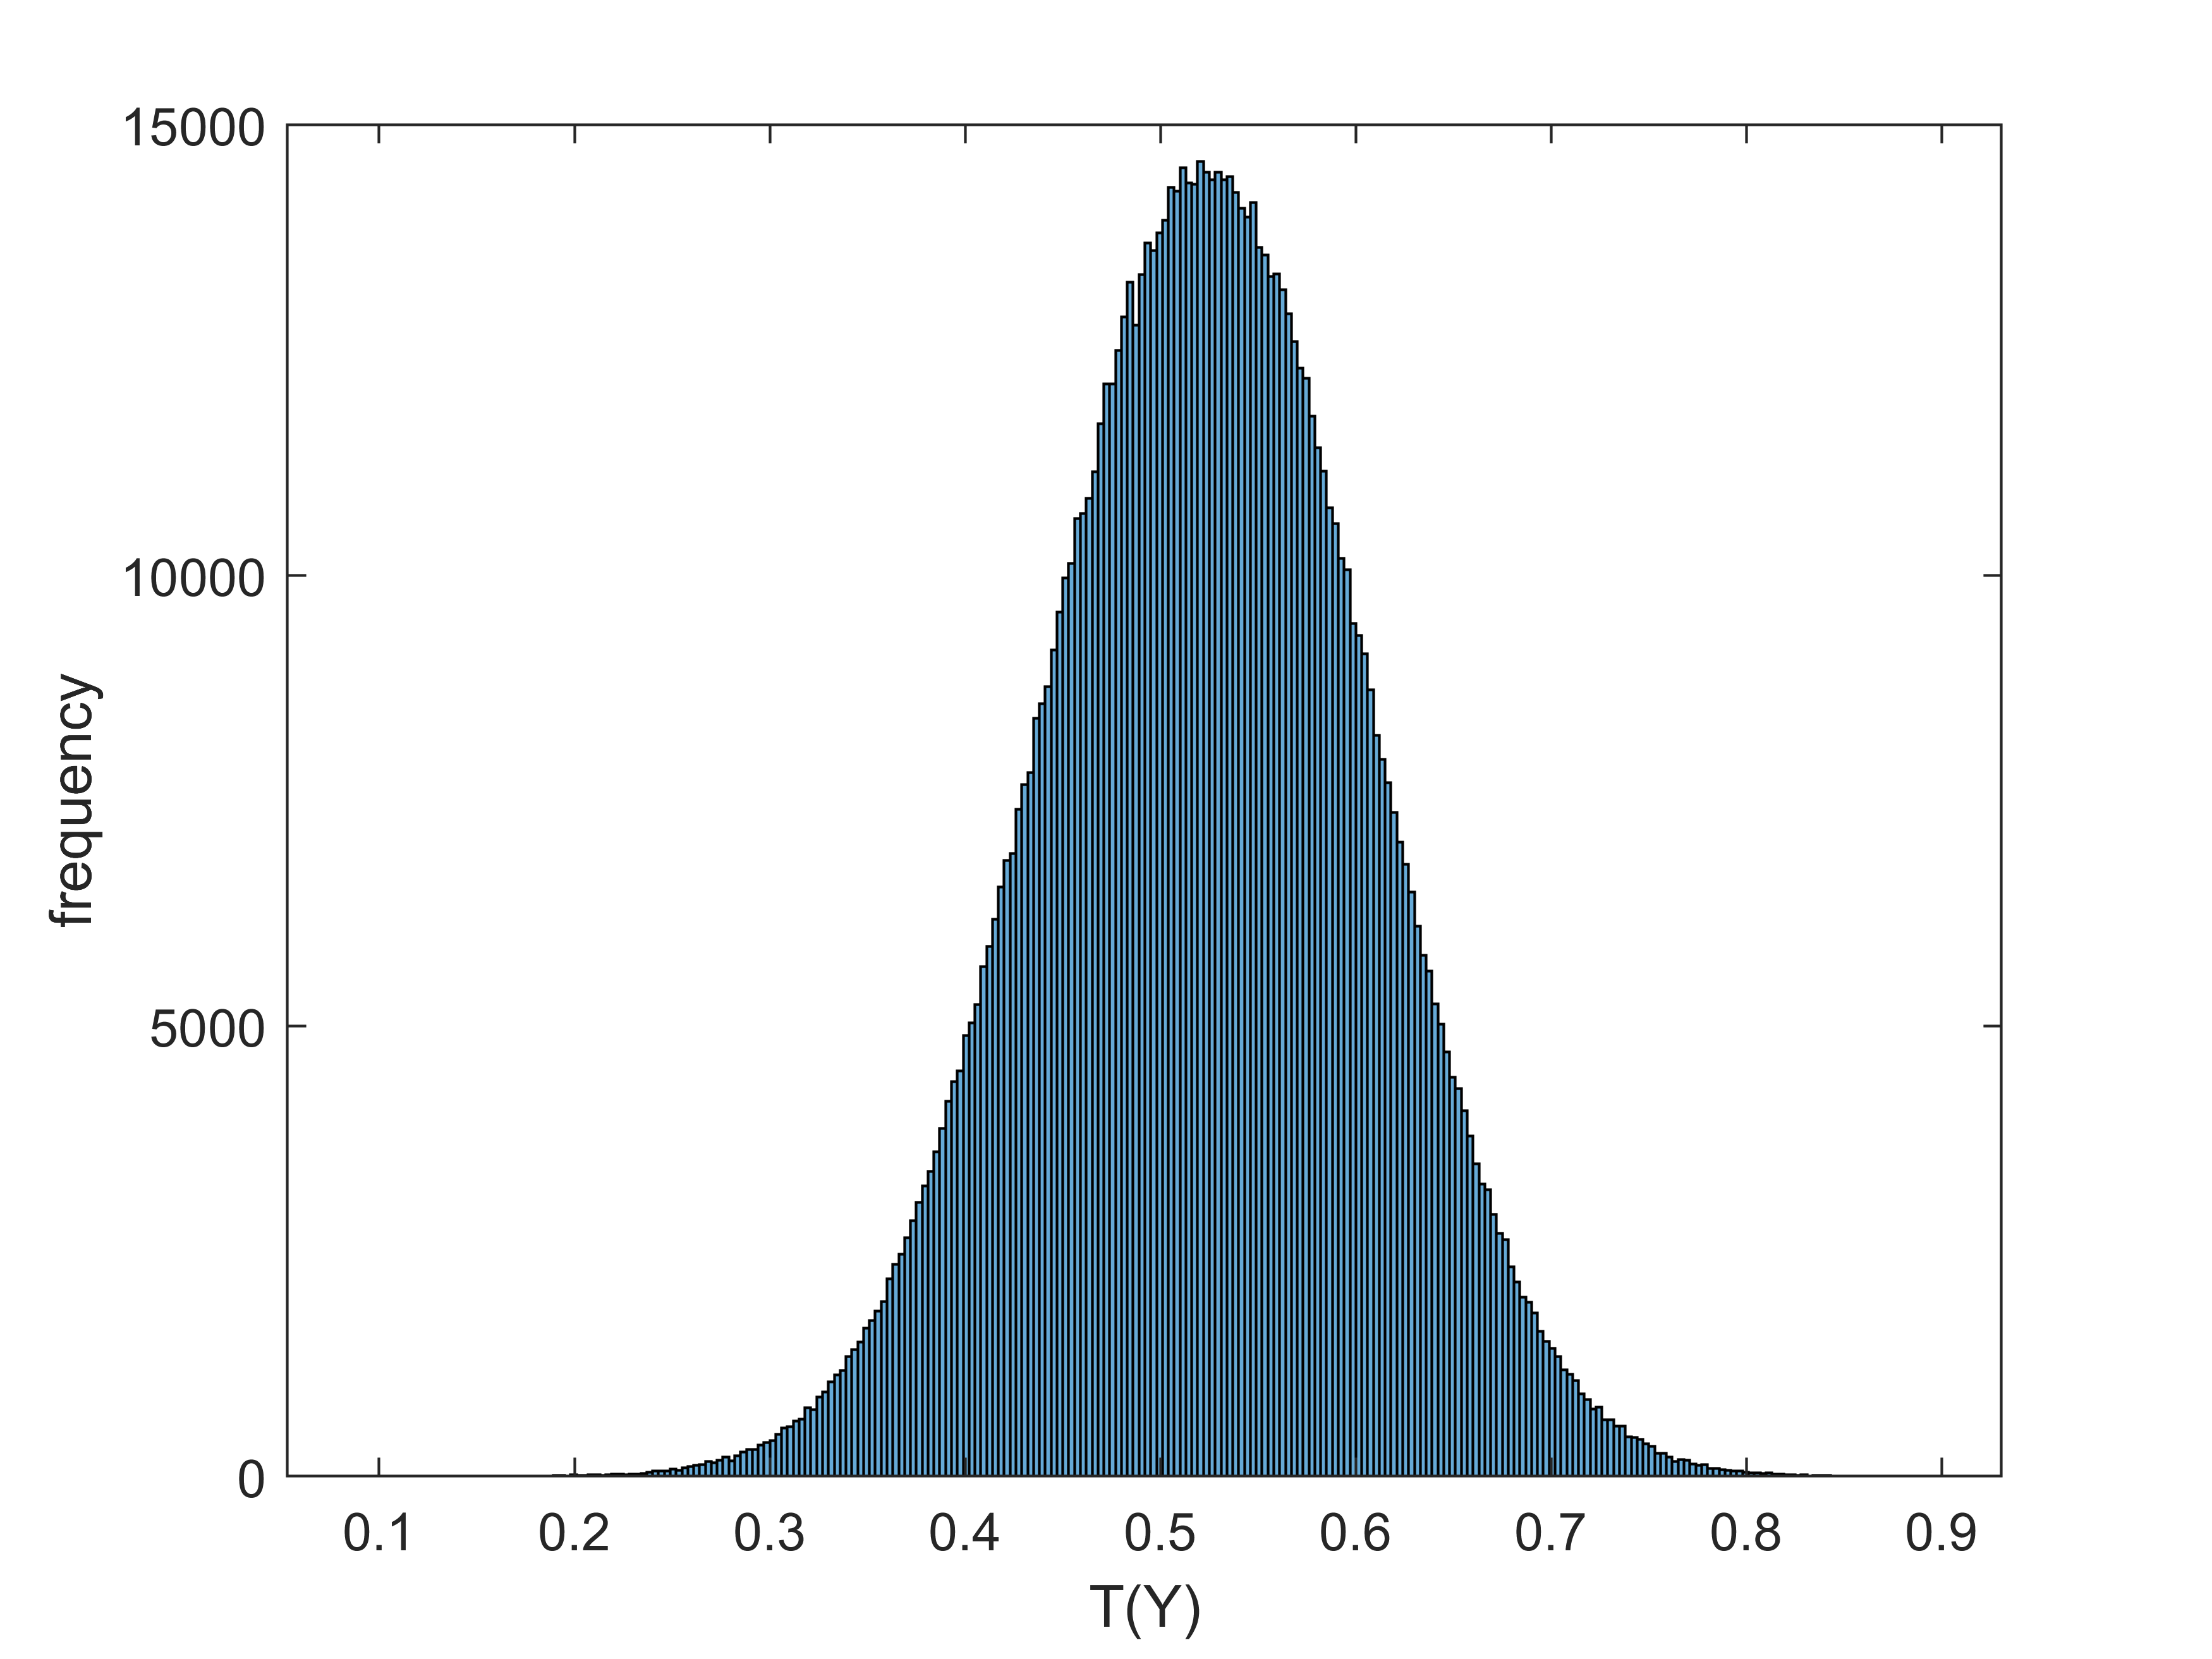
\includegraphics[width=\textwidth]{files/q2_histogram.png}
            \caption{histogram of $T(\mathbf{Y}_b)$ for $B=10^6$}
        \end{minipage}
        \hfill
        \begin{minipage}[b]{0.47\linewidth}
            \centering
            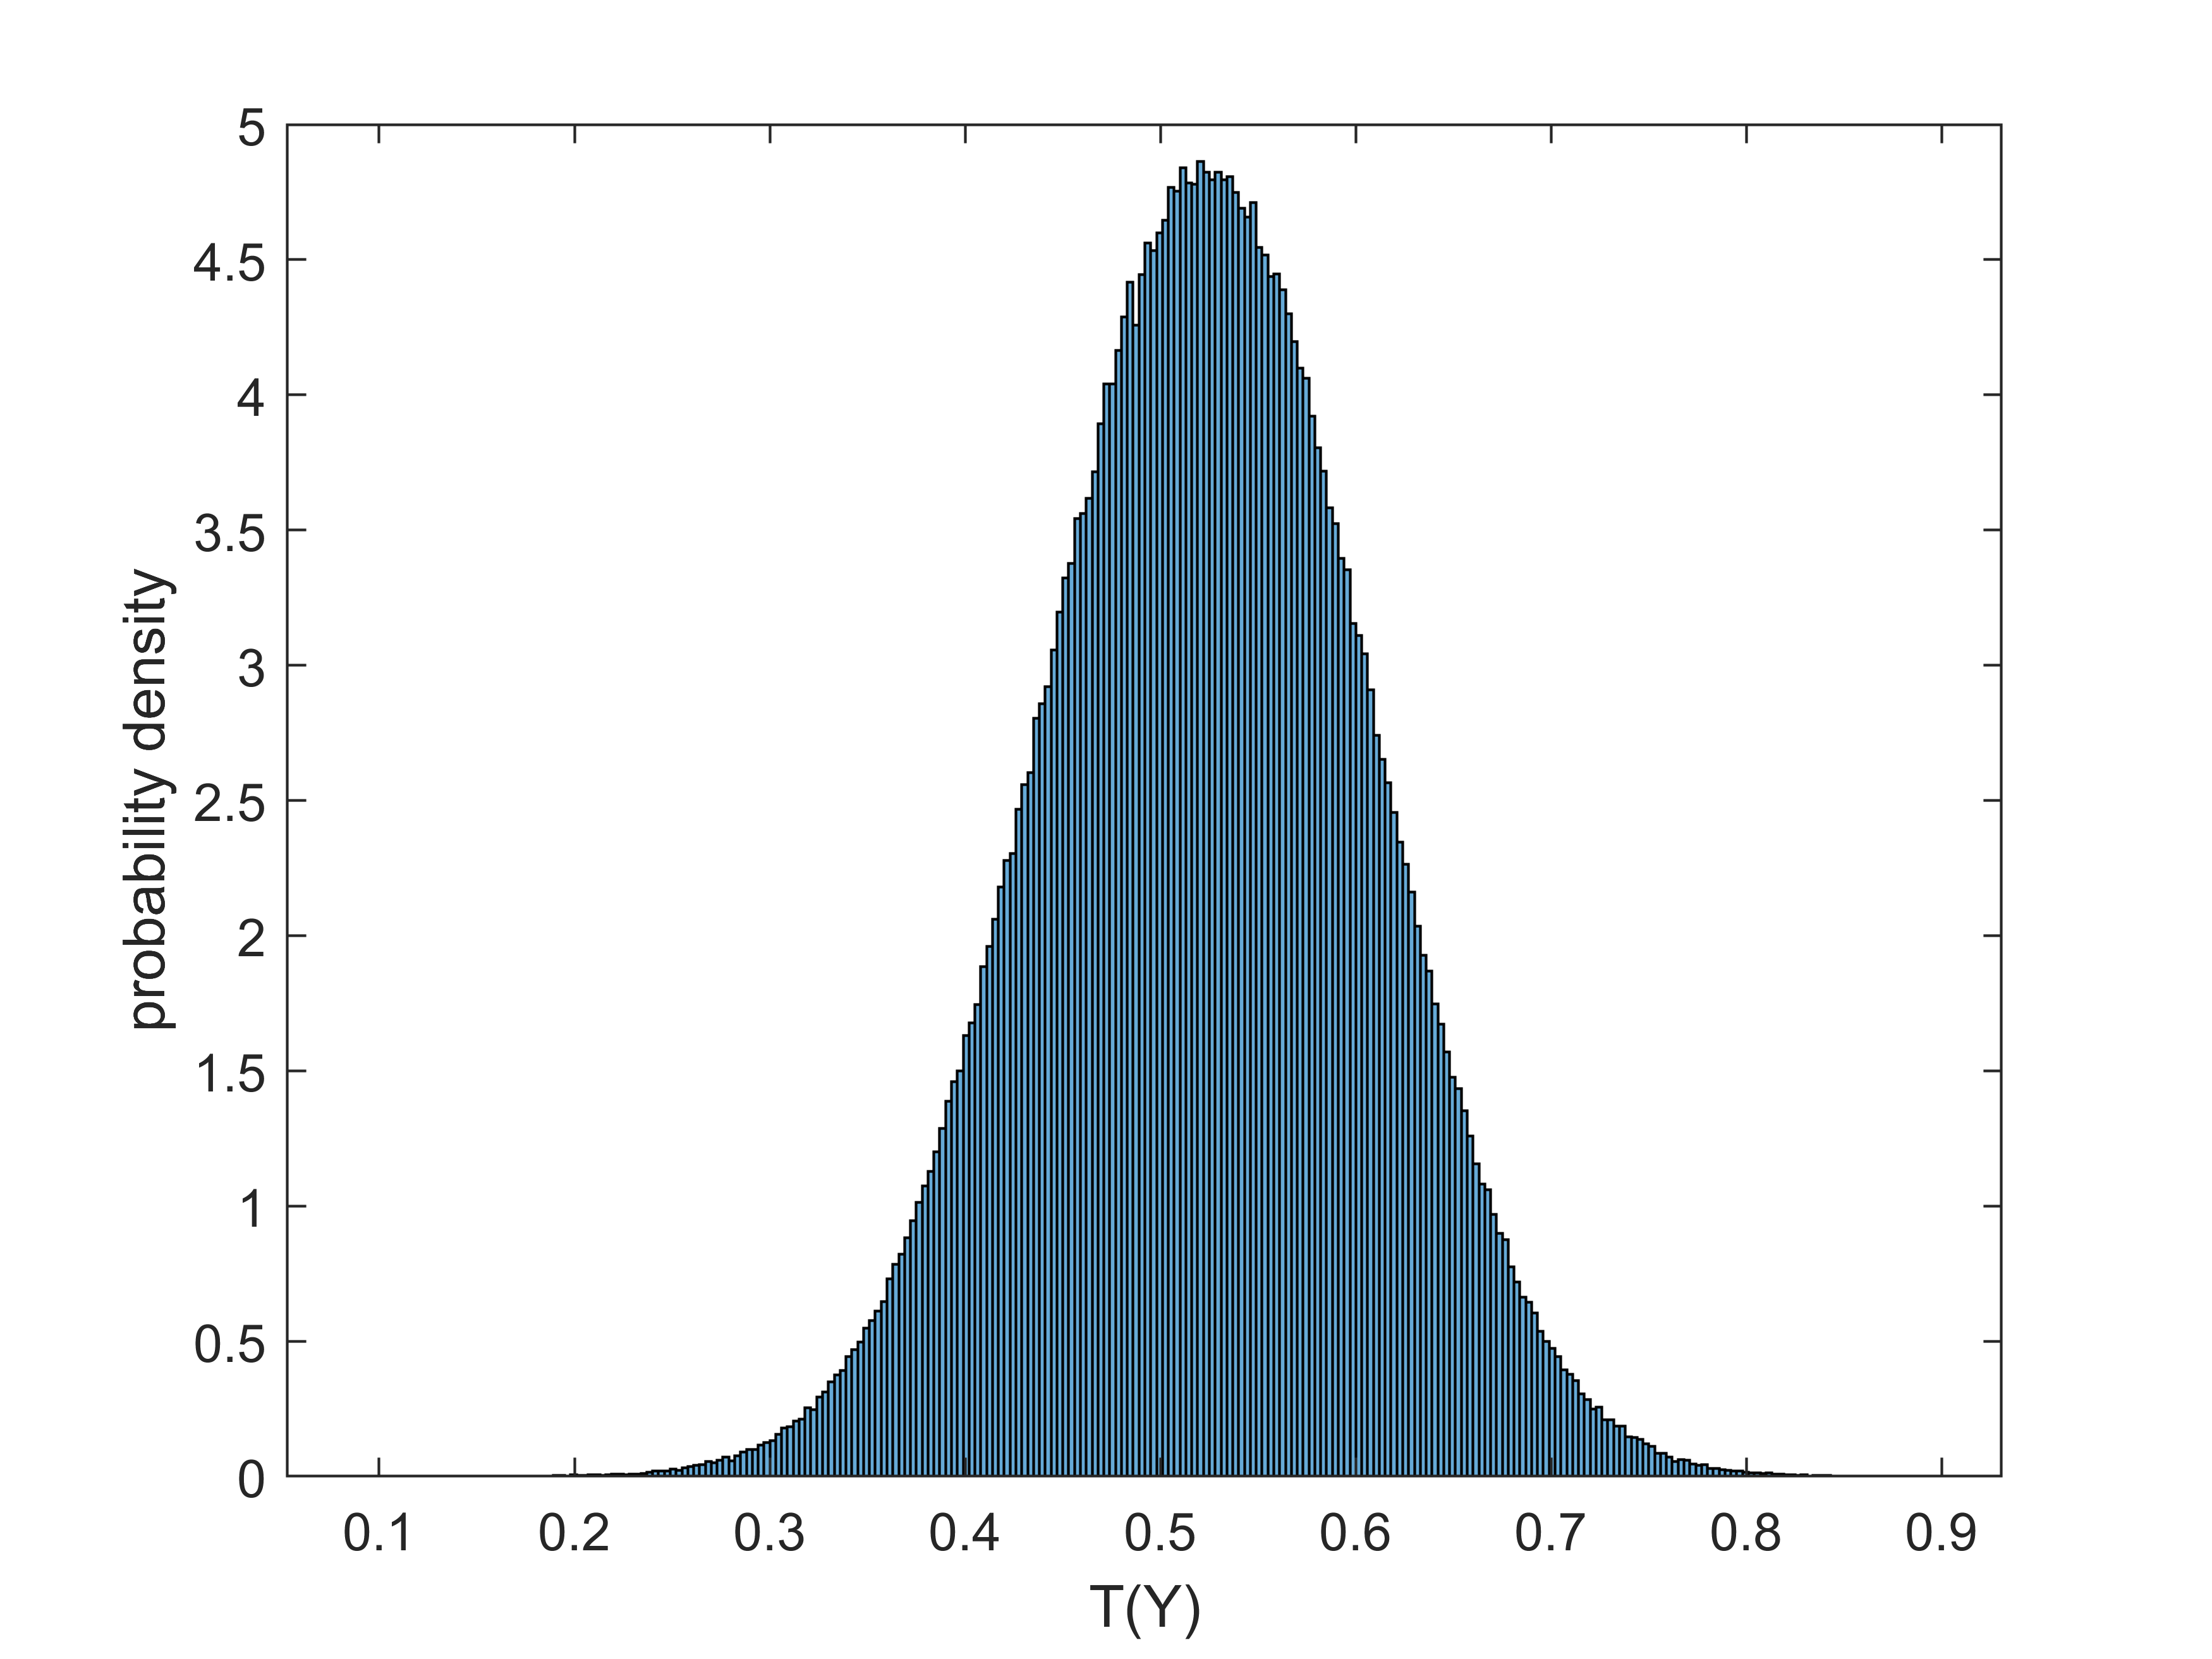
\includegraphics[width=\textwidth]{files/q2_pdf.png}
            \caption{histogram of $T(\mathbf{Y}_b)$ normalised as pdf}
        \end{minipage}
\end{figure}
\noindent The left figure is the original histogram and the right is the histogram normalised as a probability density function.\\
The mean of the graph is $0.5229$, the variance is $0.0068$, the minimum is $0.0941$ and the maximum is $0.9140$. An interesting feature of the graph is that its symmetrical around its mean at $0.5229$, and the frequency/probability density of the distribution rapidly decreases as $|t-0.5229|$ increases.\\
These are signs that $T$ might follow a normal distribution. We can try to verify this by plotting a normal distribution $N(0.5229, 0.0068)$ over the pdf-normalised version of the histogram. (figure 3)\\
\begin{figure}[H]
\centering
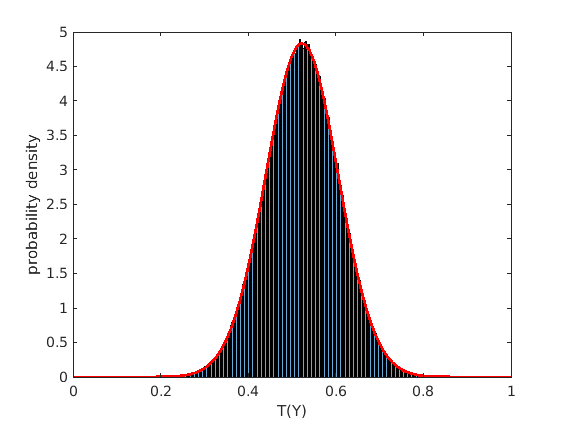
\includegraphics[width=0.47\textwidth]{files/q2_normal.png}
\caption{normal distribution and distribution of $T(\mathbf{T}_b)$}
\end{figure}
\noindent To achieve this, we enter the following lines in the command window after running \emph{'i) q2 \textunderscore bootstrap.m'}.
\begin{lstlisting}
x = [0:0.01:1];
y = normpdf(x,0.5229,sqrt(0.0068)); 
hold on
plot(x,y,'Linewidth',2,'Color','r')
\end{lstlisting}
We can see in figure 3 that the normal distribution pdf fits the pdf of $T(\mathbf{Y}_b)$ almost perfectly, this implies that $T(\mathbf{Y}_b)$ is very likely to be normally distributed with parameters $(\mu,\sigma^2)=(0.5229,0.0068)$.


\subsection*{Question 3}
To estimate $\sigma(T;F)$, we attempt to find the best estimation for $\sigma(T;\hat{F})$. We do this by using the program \emph{'ii) q3.m'}.\\
In the code, we first calculate $T(\mathbf{Y}_b)$ for $B$ times, and find $\hat{\sigma}_B$. We then repeat this $k$ times and plot a histogram of $\hat{\sigma}_B$ to show its distribution.\\
By theory, as $B\to\infty$, $\hat{\sigma}_B\to\sigma(T;\hat{F})$, so ideally we would want $B$ to be as large as possible, since this would give us the best approximation of $\sigma(T;\hat{F})$.
In implementation, if we choose $B$ to be too large then it's computationally slow to calculate with a large $k$. We can show this by finding the time complexity of calculating $\hat{\sigma}_B$.\\
Drawing one bootstrap sample $\mathbf{Y}_b$ has complexity $\mathcal{O}(N)$ where $N$ is the number of data points. Calculating $\Bar{Y}$ and $\Bar{Z}$ has complexity $\mathcal{O}(N)$, but we can cache them so that we don't need to calculate them again when finding $r(\mathbf{Y}_b)$.\\
So $\sum(Y_i-\Bar{Y})(Z_i-\Bar{Z})$ is just $N\cdot\mathcal{O}(1)$ and $\sqrt{\sum(Y_i-\Bar{Y})^2}$ is also $N\cdot\mathcal{O}(1)$.\\
Hence, $r(\mathbf{Y}_b)$ has time complexity $4*\mathcal{O}(N)=\mathcal{O}(N)$. So $T(\mathbf{Y}_b)$ is $\mathcal{O}(N)$.\\
Similarly, $\Bar{T}$ is $\mathcal{O}(B)$ and $\hat{\sigma}_B$ has complexity $B*\mathcal{O}(N)=\mathcal{O}(BN)$.\\
We are repeating this $k$ times, so the total time complexity of the algorithm is $k\cdot (\mathcal{O}(BN)+\mathcal{O}(B))=\mathcal{O}(kBN)$.\\
In our case, $N$ is fixed to $120$, so the time taken is only dependent on $B$ and $k$, and the time required to execute the program is linearly proportional to the size of $B$.\\
Hence, we consider $B=10^3,10^4,10^5$ with $k=1000$ to plot the histograms.
\begin{figure}[H]
    \begin{minipage}[b]{0.47\linewidth}
            \centering
            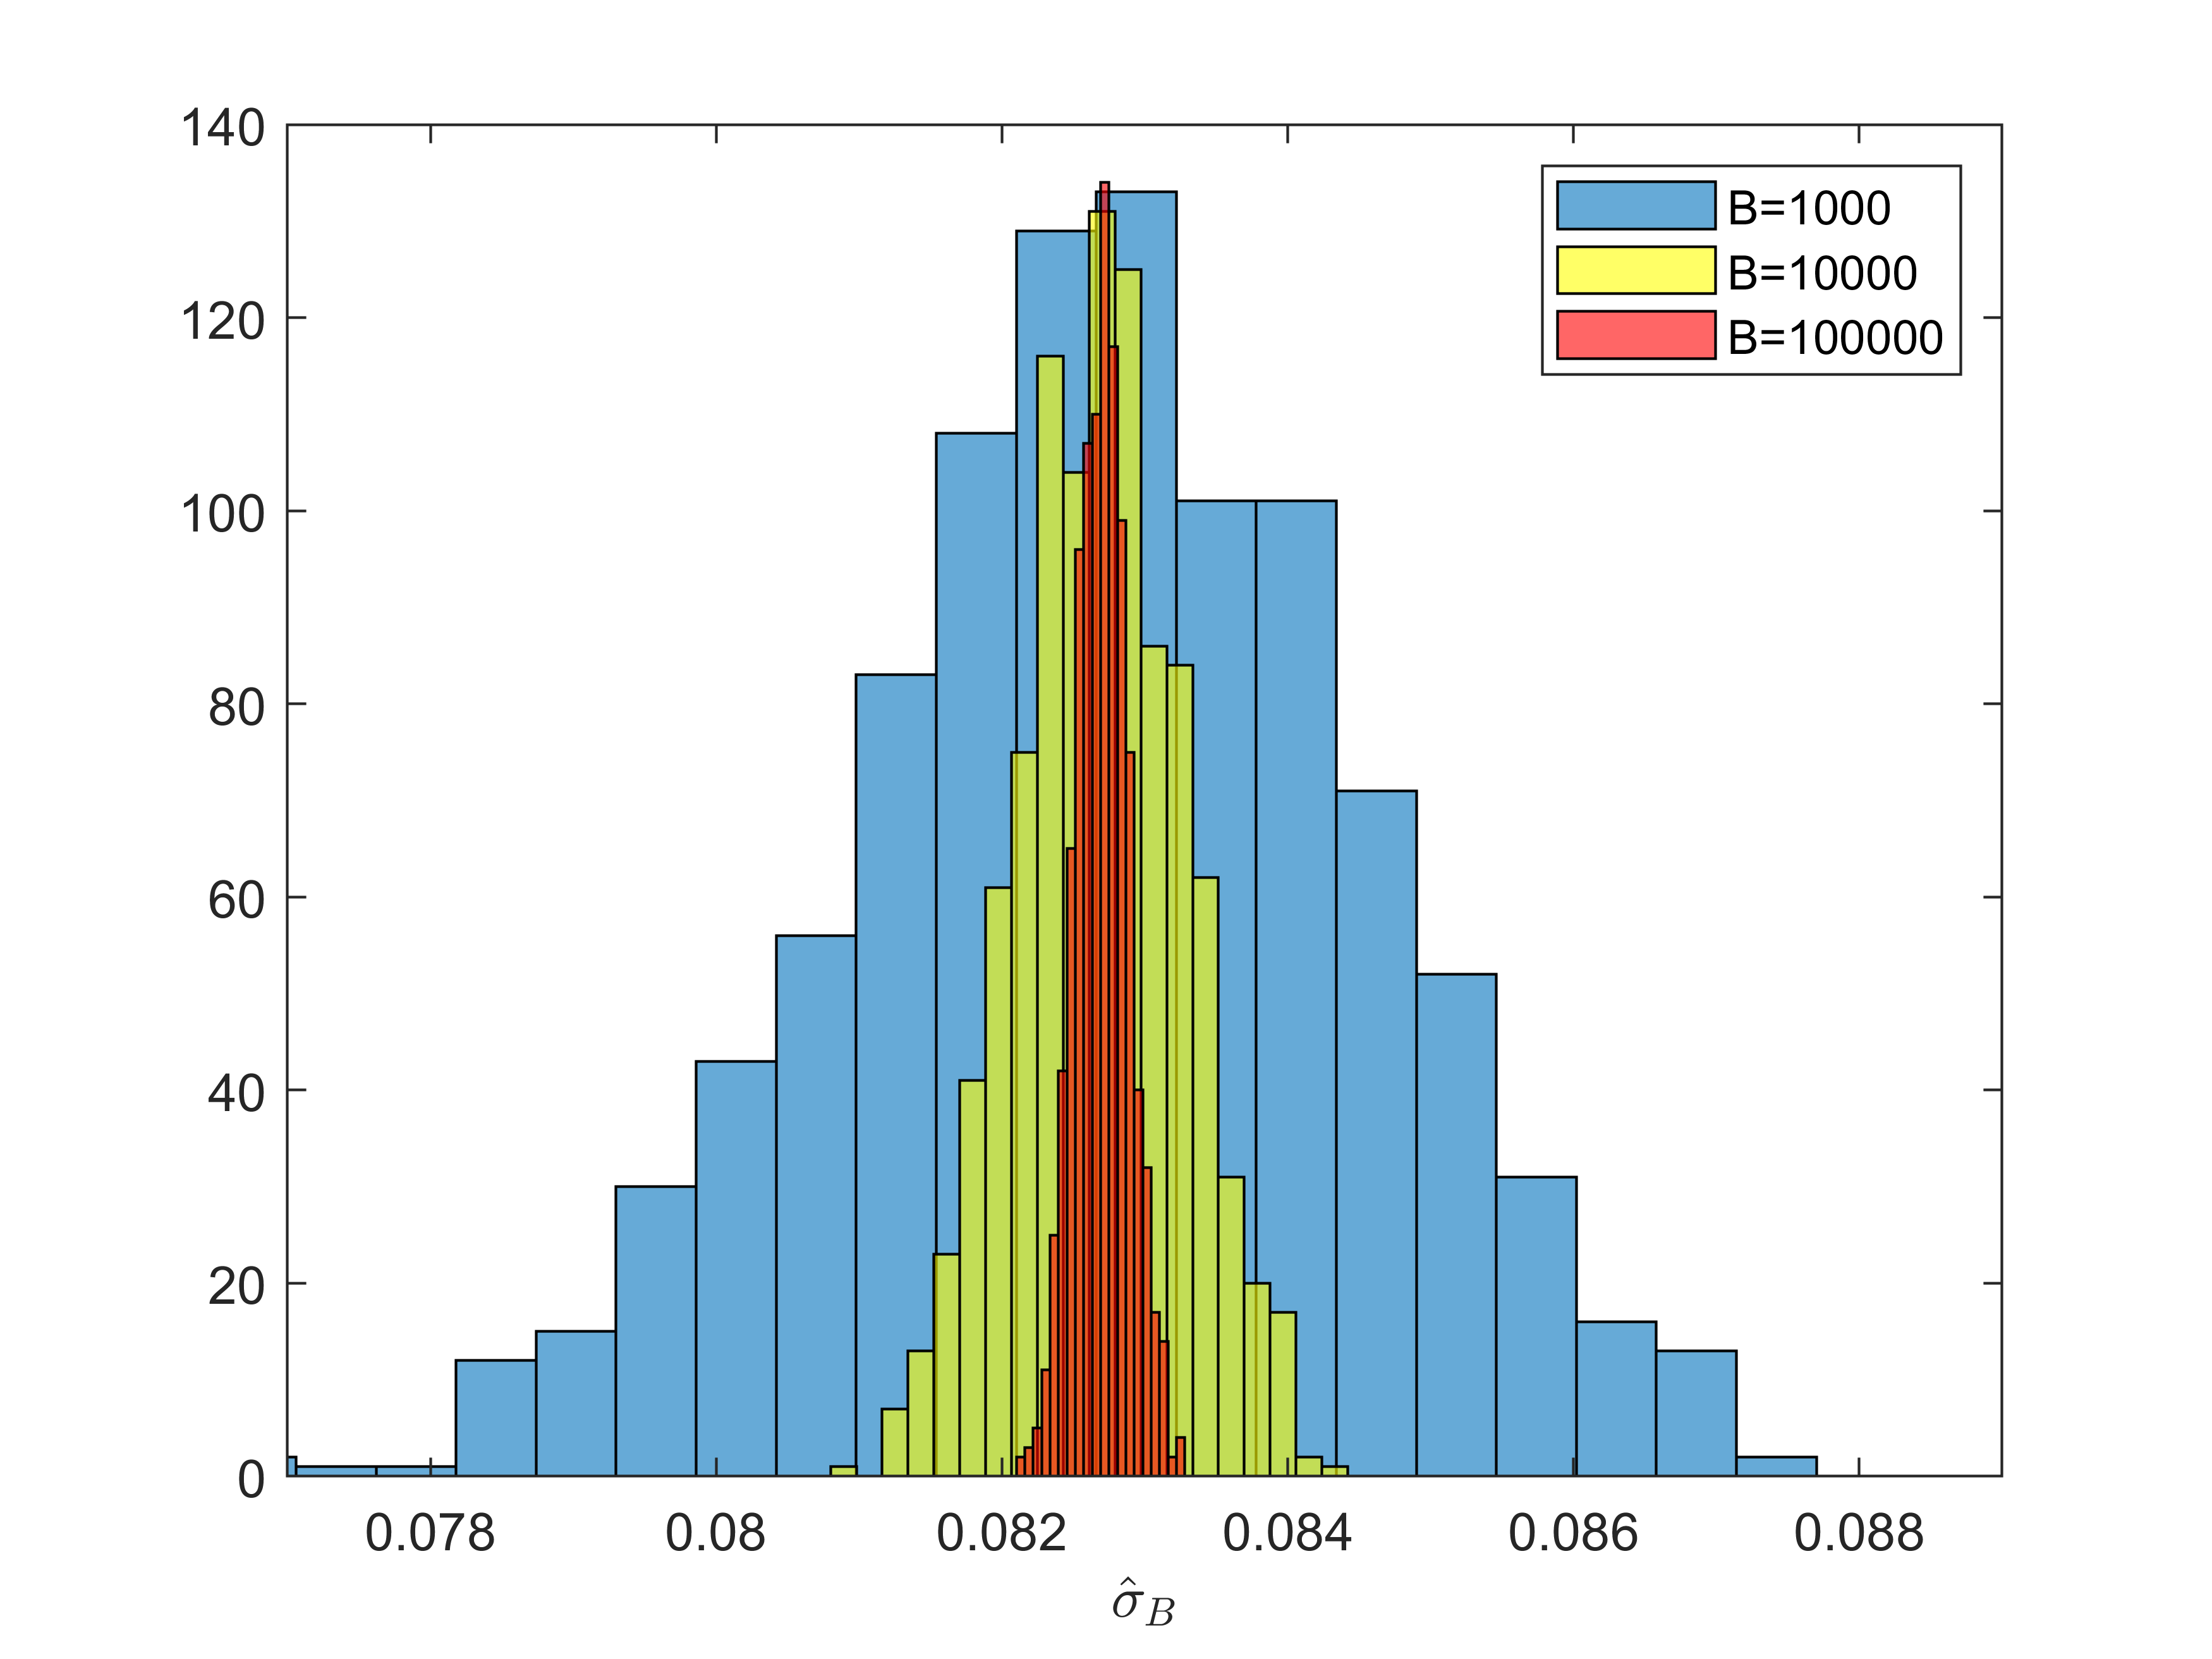
\includegraphics[width=\textwidth]{files/q3.png}
            \caption{histogram of $\hat{\sigma}_B$ for range of $B$}
        \end{minipage}
        \hfill
    \begin{minipage}[b]{0.47\linewidth}
            \centering
            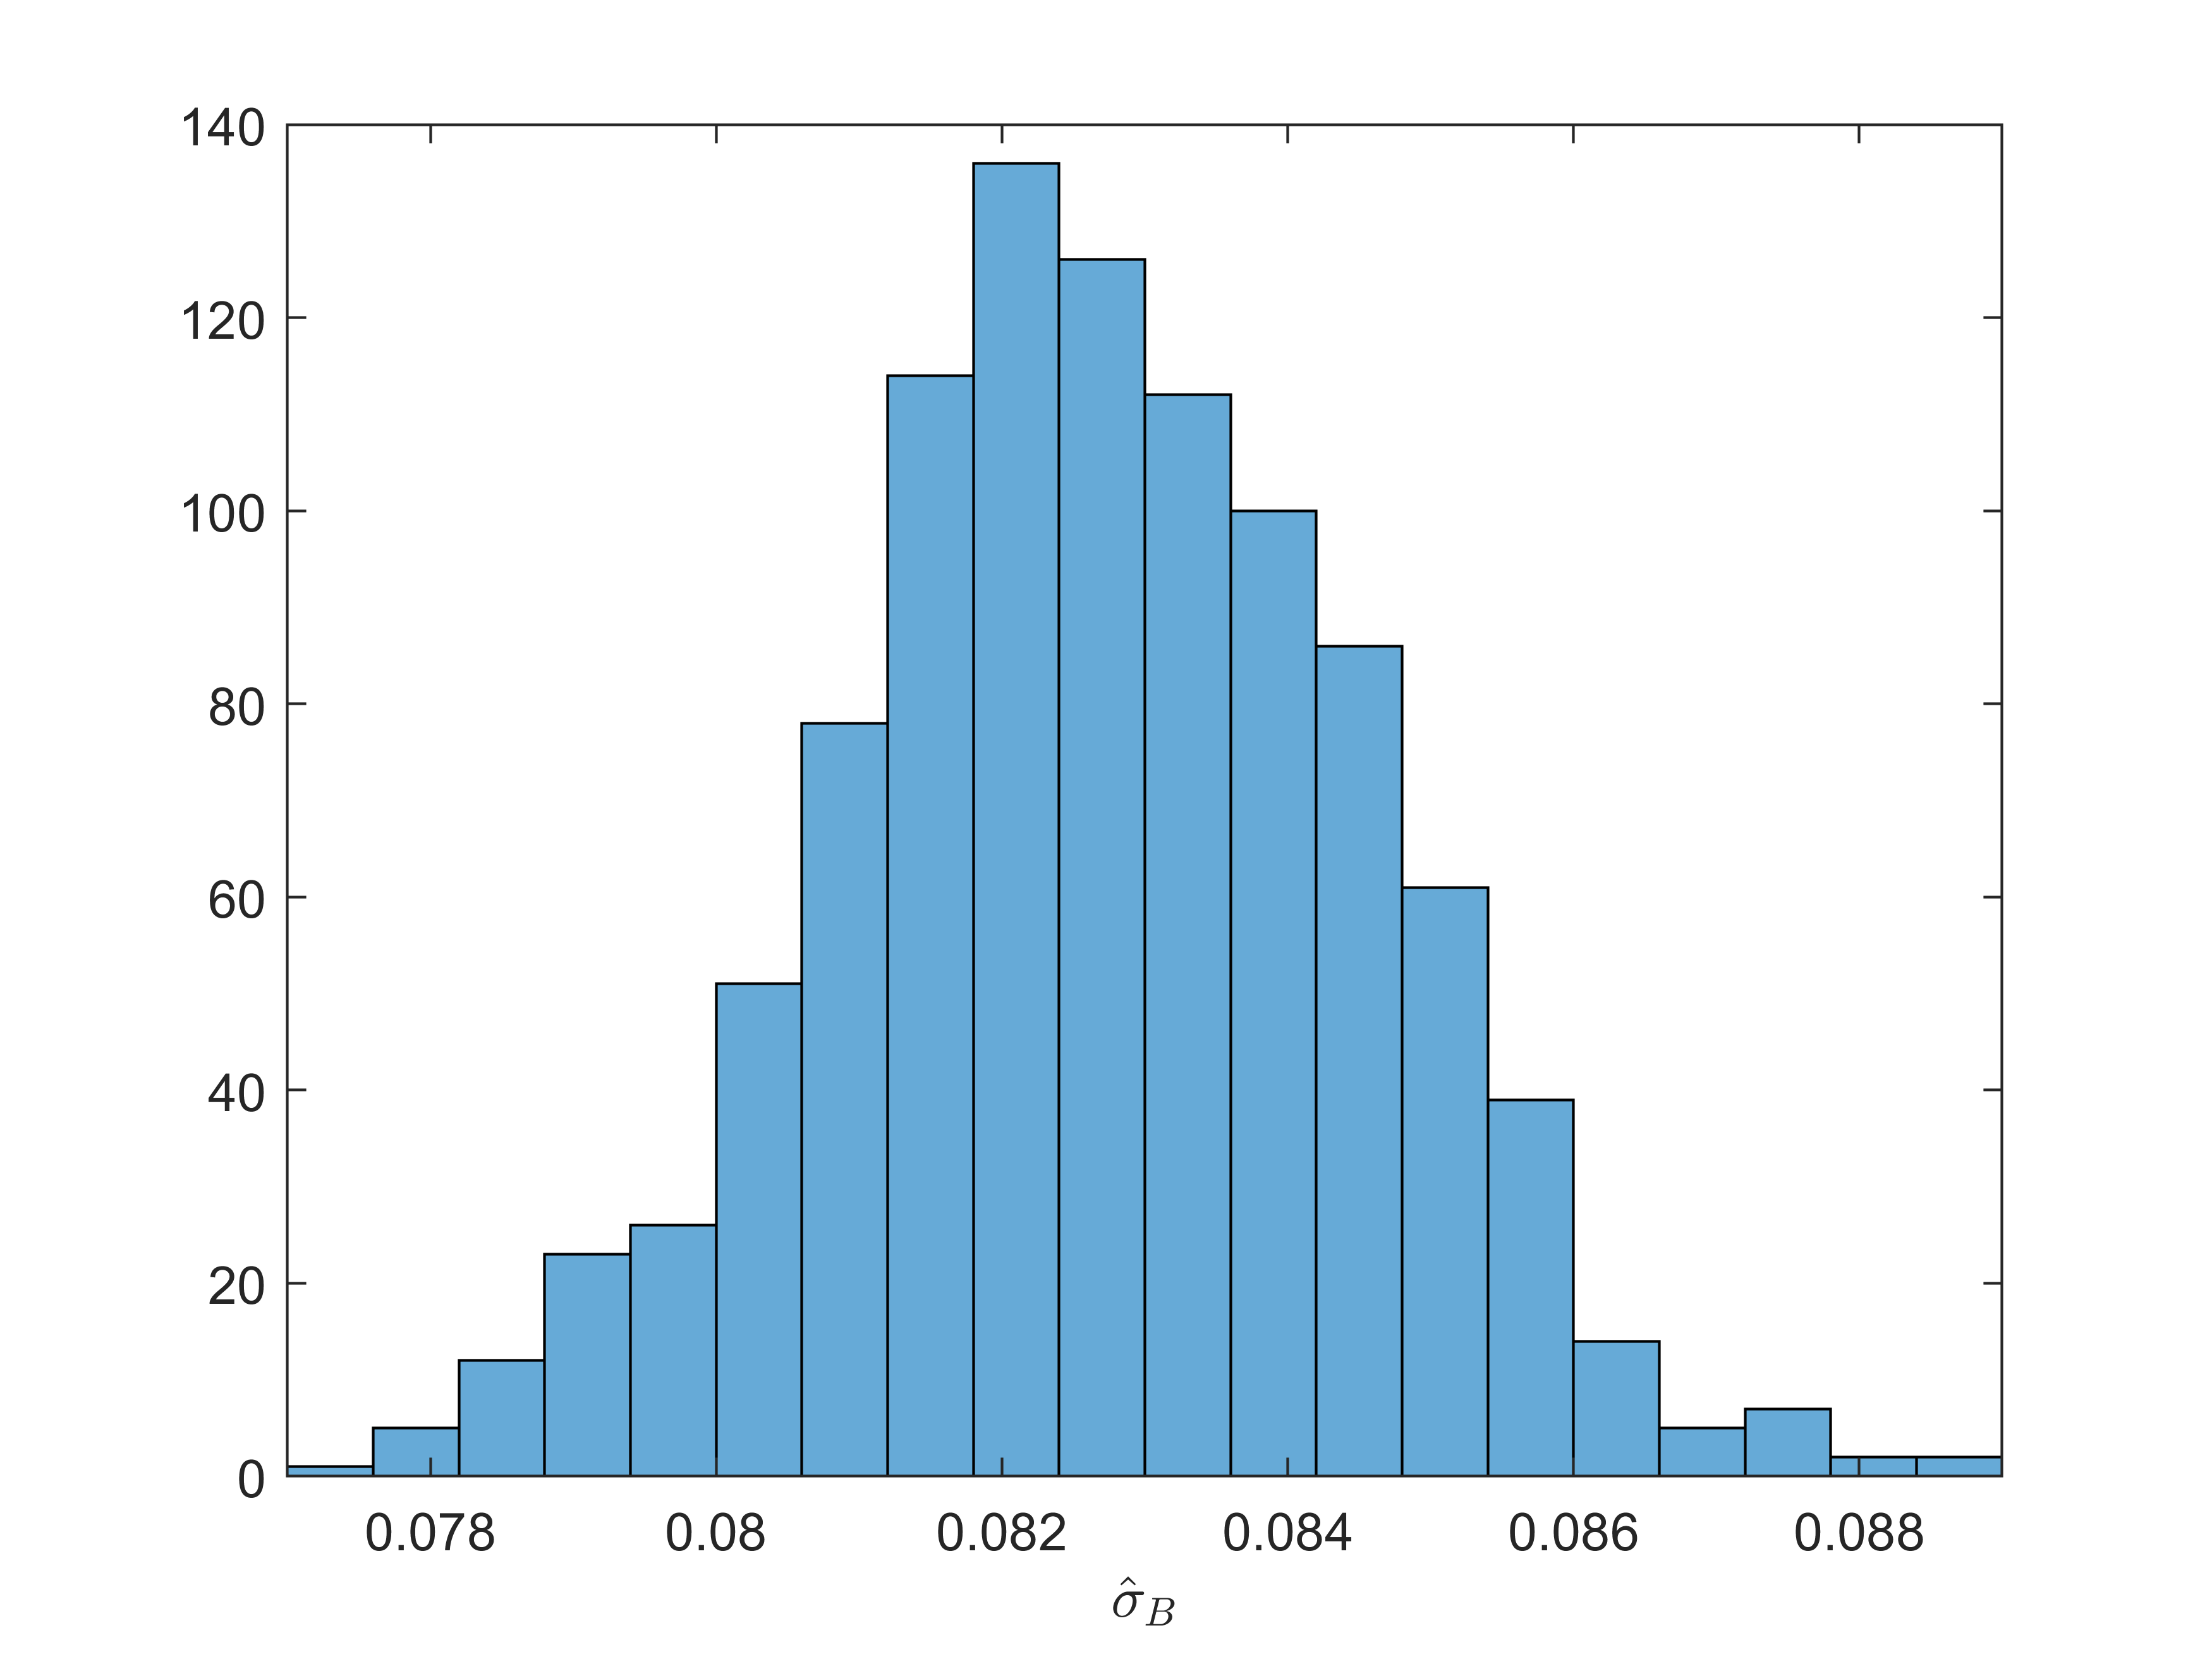
\includegraphics[width=\textwidth]{files/q3,b=10^3.png}
            \caption{histogram of $\hat{\sigma}_B$ for $B=10^3,k=1000$}
        \end{minipage}
\end{figure}
\begin{figure}[H]
    \begin{minipage}[b]{0.47\linewidth}
            \centering
            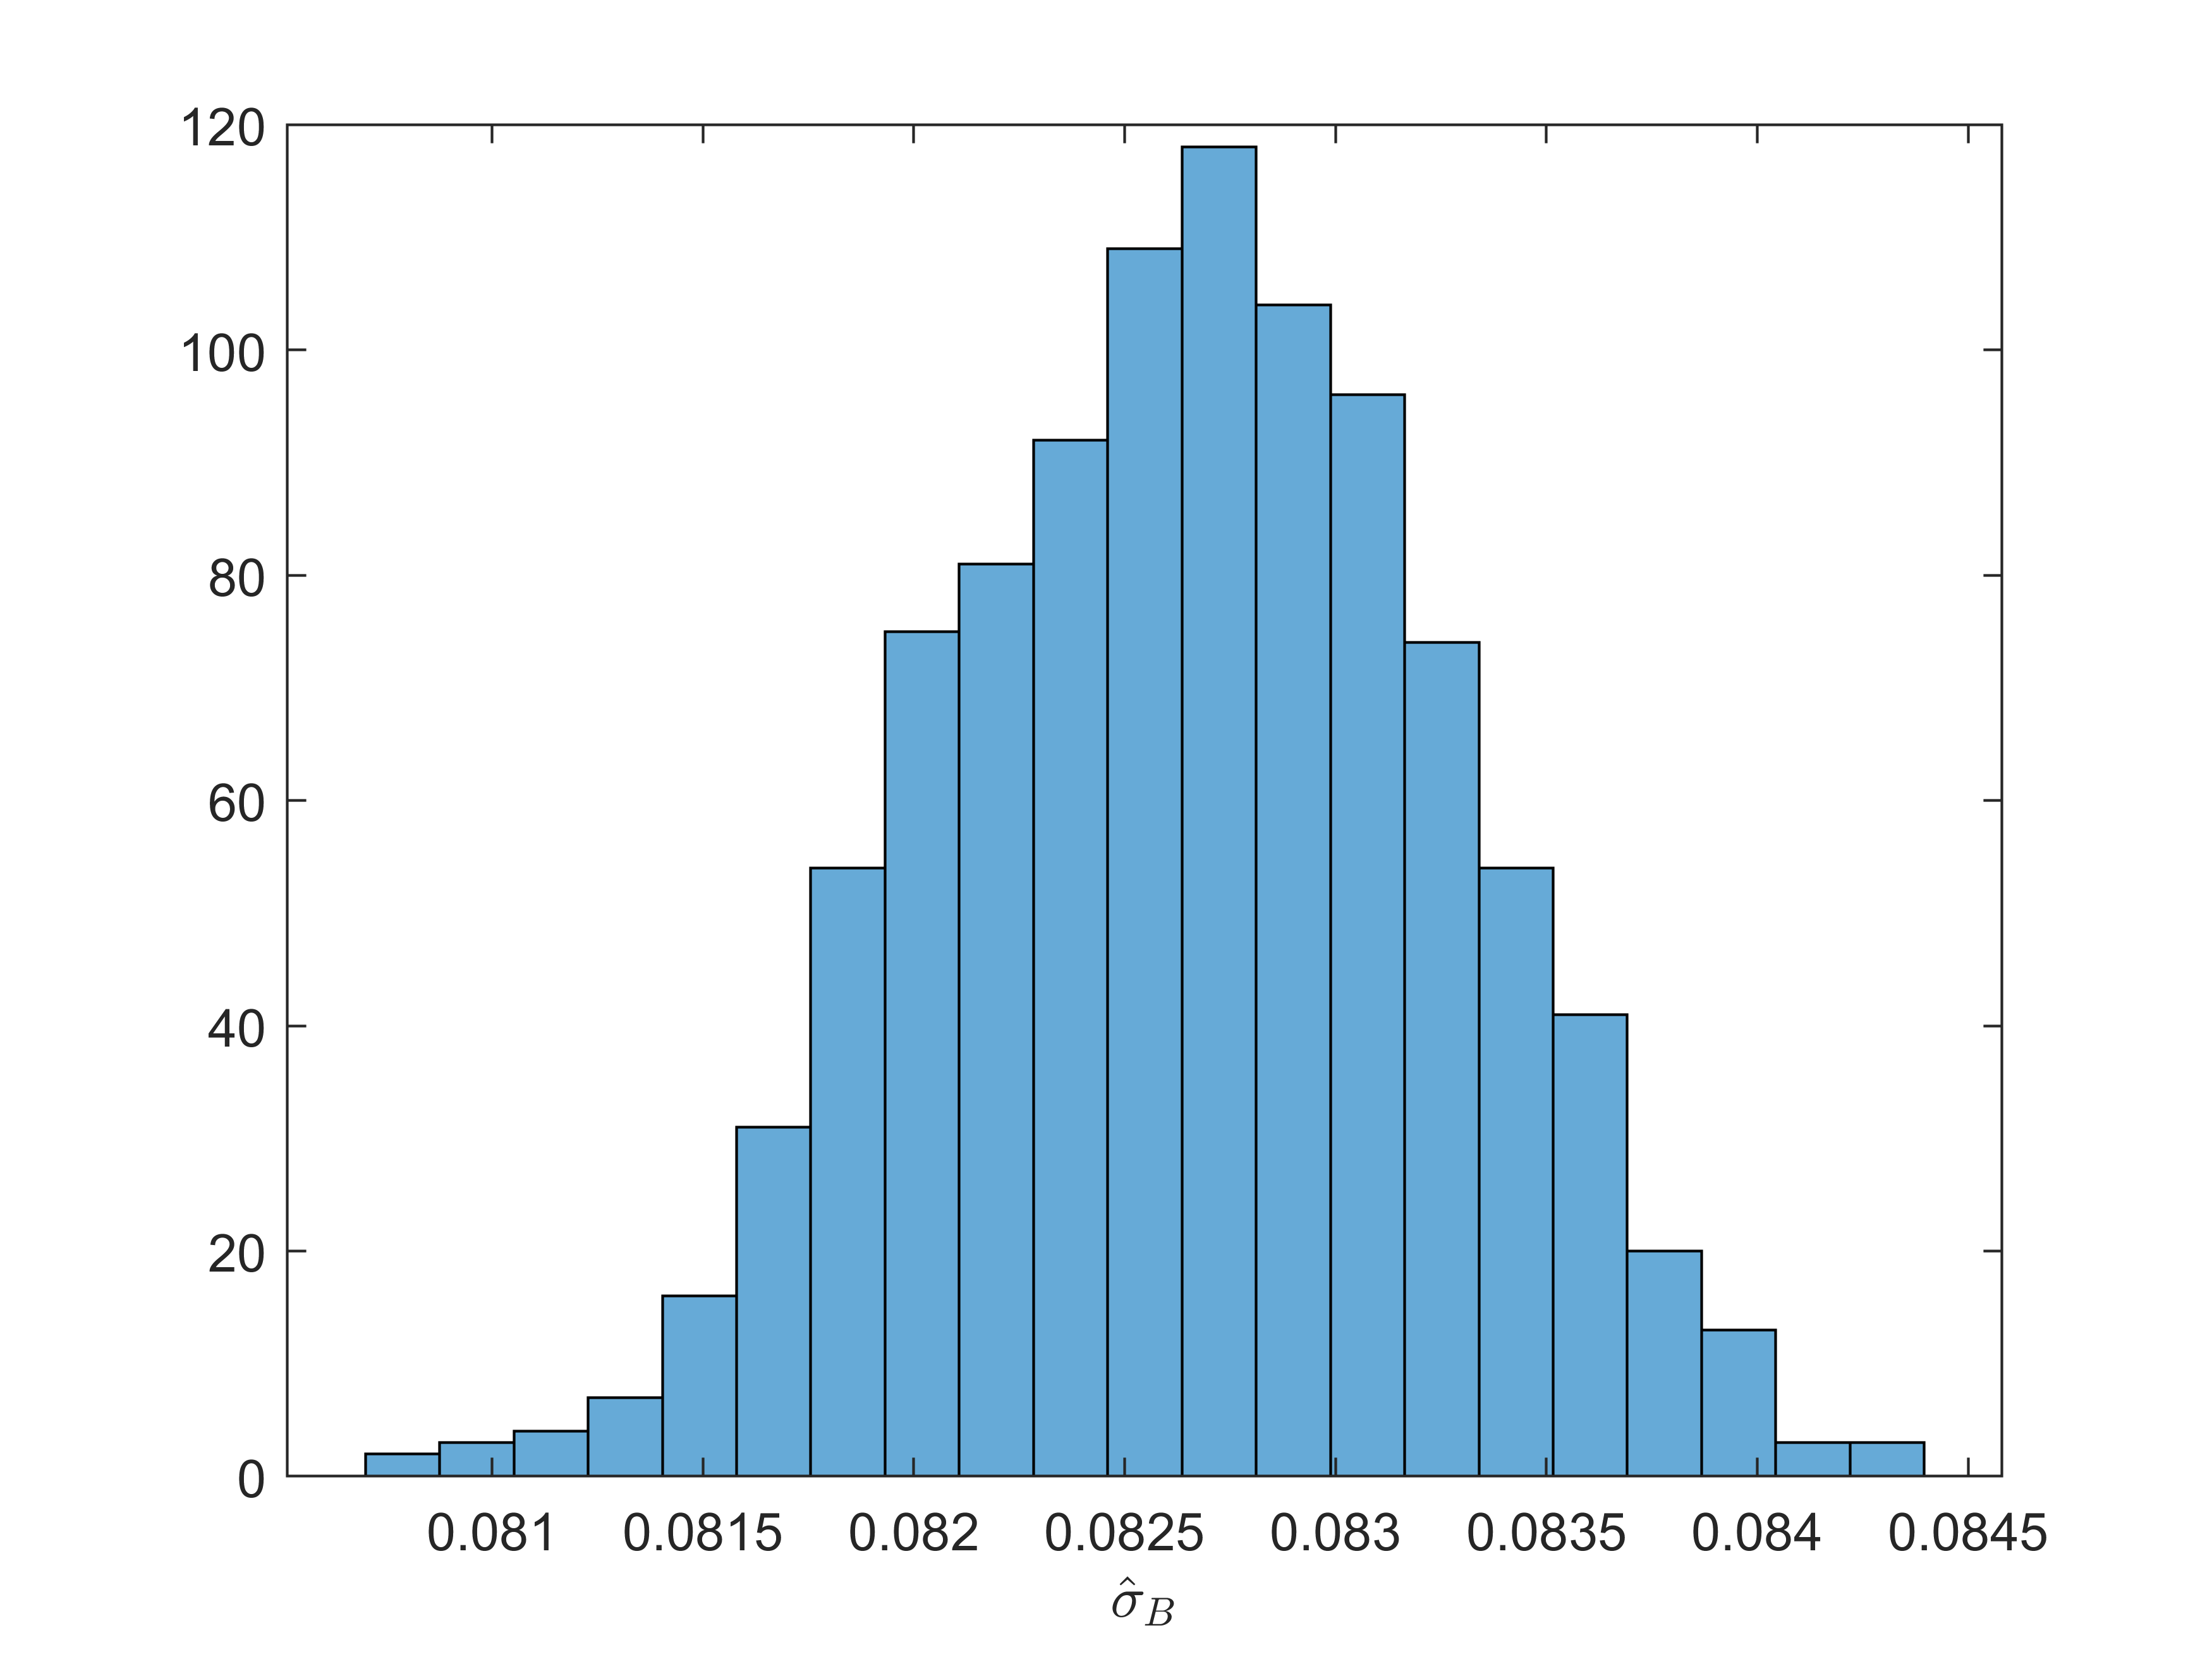
\includegraphics[width=\textwidth]{files/q3,b=10^4.png}
            \caption{histogram of $\hat{\sigma}_B$ for $B=10^4,k=1000$}
        \end{minipage}
        \hfill
        \begin{minipage}[b]{0.47\linewidth}
            \centering
            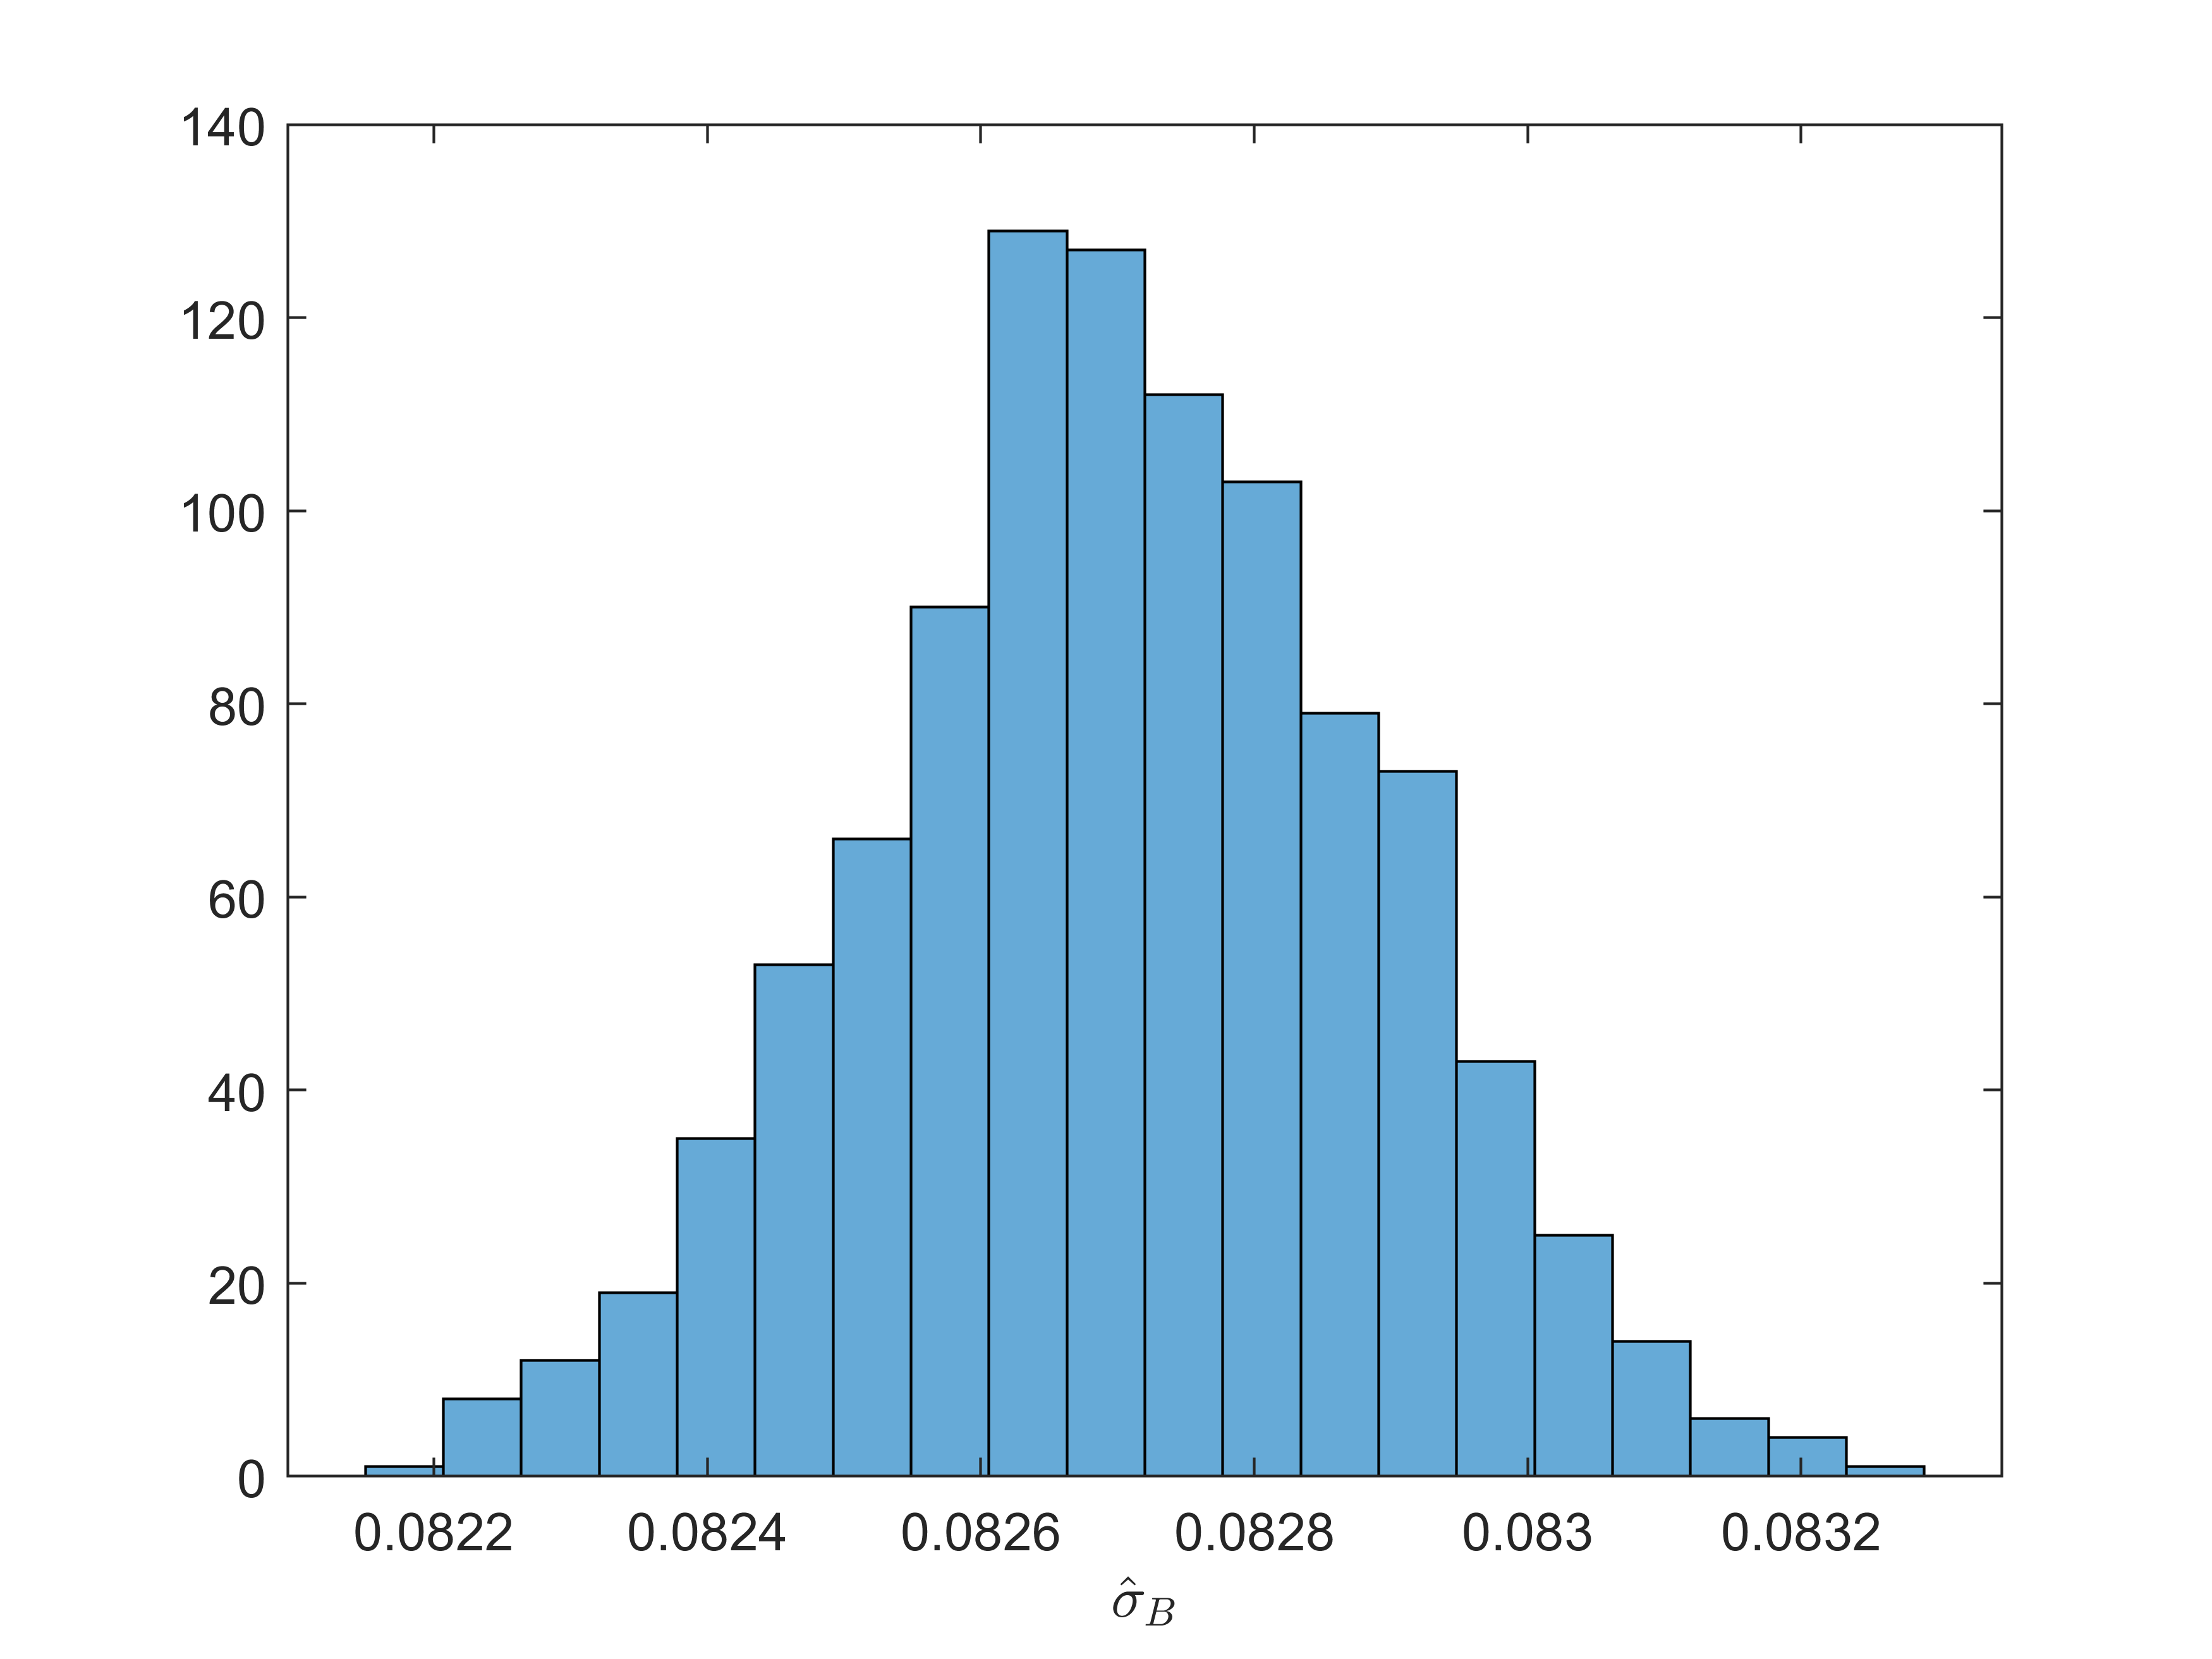
\includegraphics[width=\textwidth]{files/q3,b=10^5.png}
            \caption{histogram of $\hat{\sigma}_B$ for $B=10^5,k=1000$}
        \end{minipage}
\end{figure}
\noindent We note that the histograms for $B=10^3,10^4,10^5$ are symmetric over the mean of the histogram, and the mean remains largely unchanged as we increase the value of $B$.\\
We note also when the histograms' bin sizes are scaled with respect to their range, for all the value of $B$ we've tested, the shape of the histogram is mostly similar. Hence, the main change in the histogram is in the range of $\hat{\sigma}_B$ and how much the distribution is 'squeezed' when $B$ is increased by a factor of $10$.\\
With $k=1000$ tests, when $B=10^3$, $\hat{\sigma}_B$ ranges from $0.077$ to $0.089$; when $B=10^4$, $\hat{\sigma}_B$ ranges from $0.0805$ to $0.0844$ and when $B=10^5$, $\hat{\sigma}_B$ ranges from $0.0821$ to $0.0833$. \\
We thus note range$(\hat{\sigma}_B)|_{B=10^{k+1}}\approx\frac{1}{3}\cdot$ range$(\hat{\sigma}_B)|_{B=10^{k}}$, i.e. the rate of the errors is $\mathcal{O}(\frac{1}{\sqrt{B}})$.\\
The 'squeeze' occurs, because $\hat{\sigma}_B\to\sigma(T;\hat{F})$, and therefore $\mathds{P}(|\hat{\sigma}_B-\sigma(T;\hat{F})|> \epsilon)\to0$ as $B\to\infty$. In fact, if we assume that $T(Y)$ follows a normal distribution, then $\hat{\sigma}_B$ is the MLE for its standard error, so it's asymptotically normal with mean $\sigma(T;\hat{F})$ and the distribution's variance is proportional to $\frac{1}{B}$. Hence, the standard error has rate of errors $\mathcal{O}(\sqrt{\frac{1}{B}})=\mathcal{O}(\frac{1}{\sqrt{B}})$.\\
Therefore, I would advise to use $B=10^7$. This gives us an estimation of $\sigma(T;\hat{F})$ that's accurate to 4 d.p. and it's relatively fast to compute so we can repeat the estimation for a small $k$ and calculate the mean of the estimations to improve the accuracy.\\
So we get \underline{$\hat{\sigma}_B=0.0827$} and its histogram looks like below.
\begin{figure}[H]
\centering
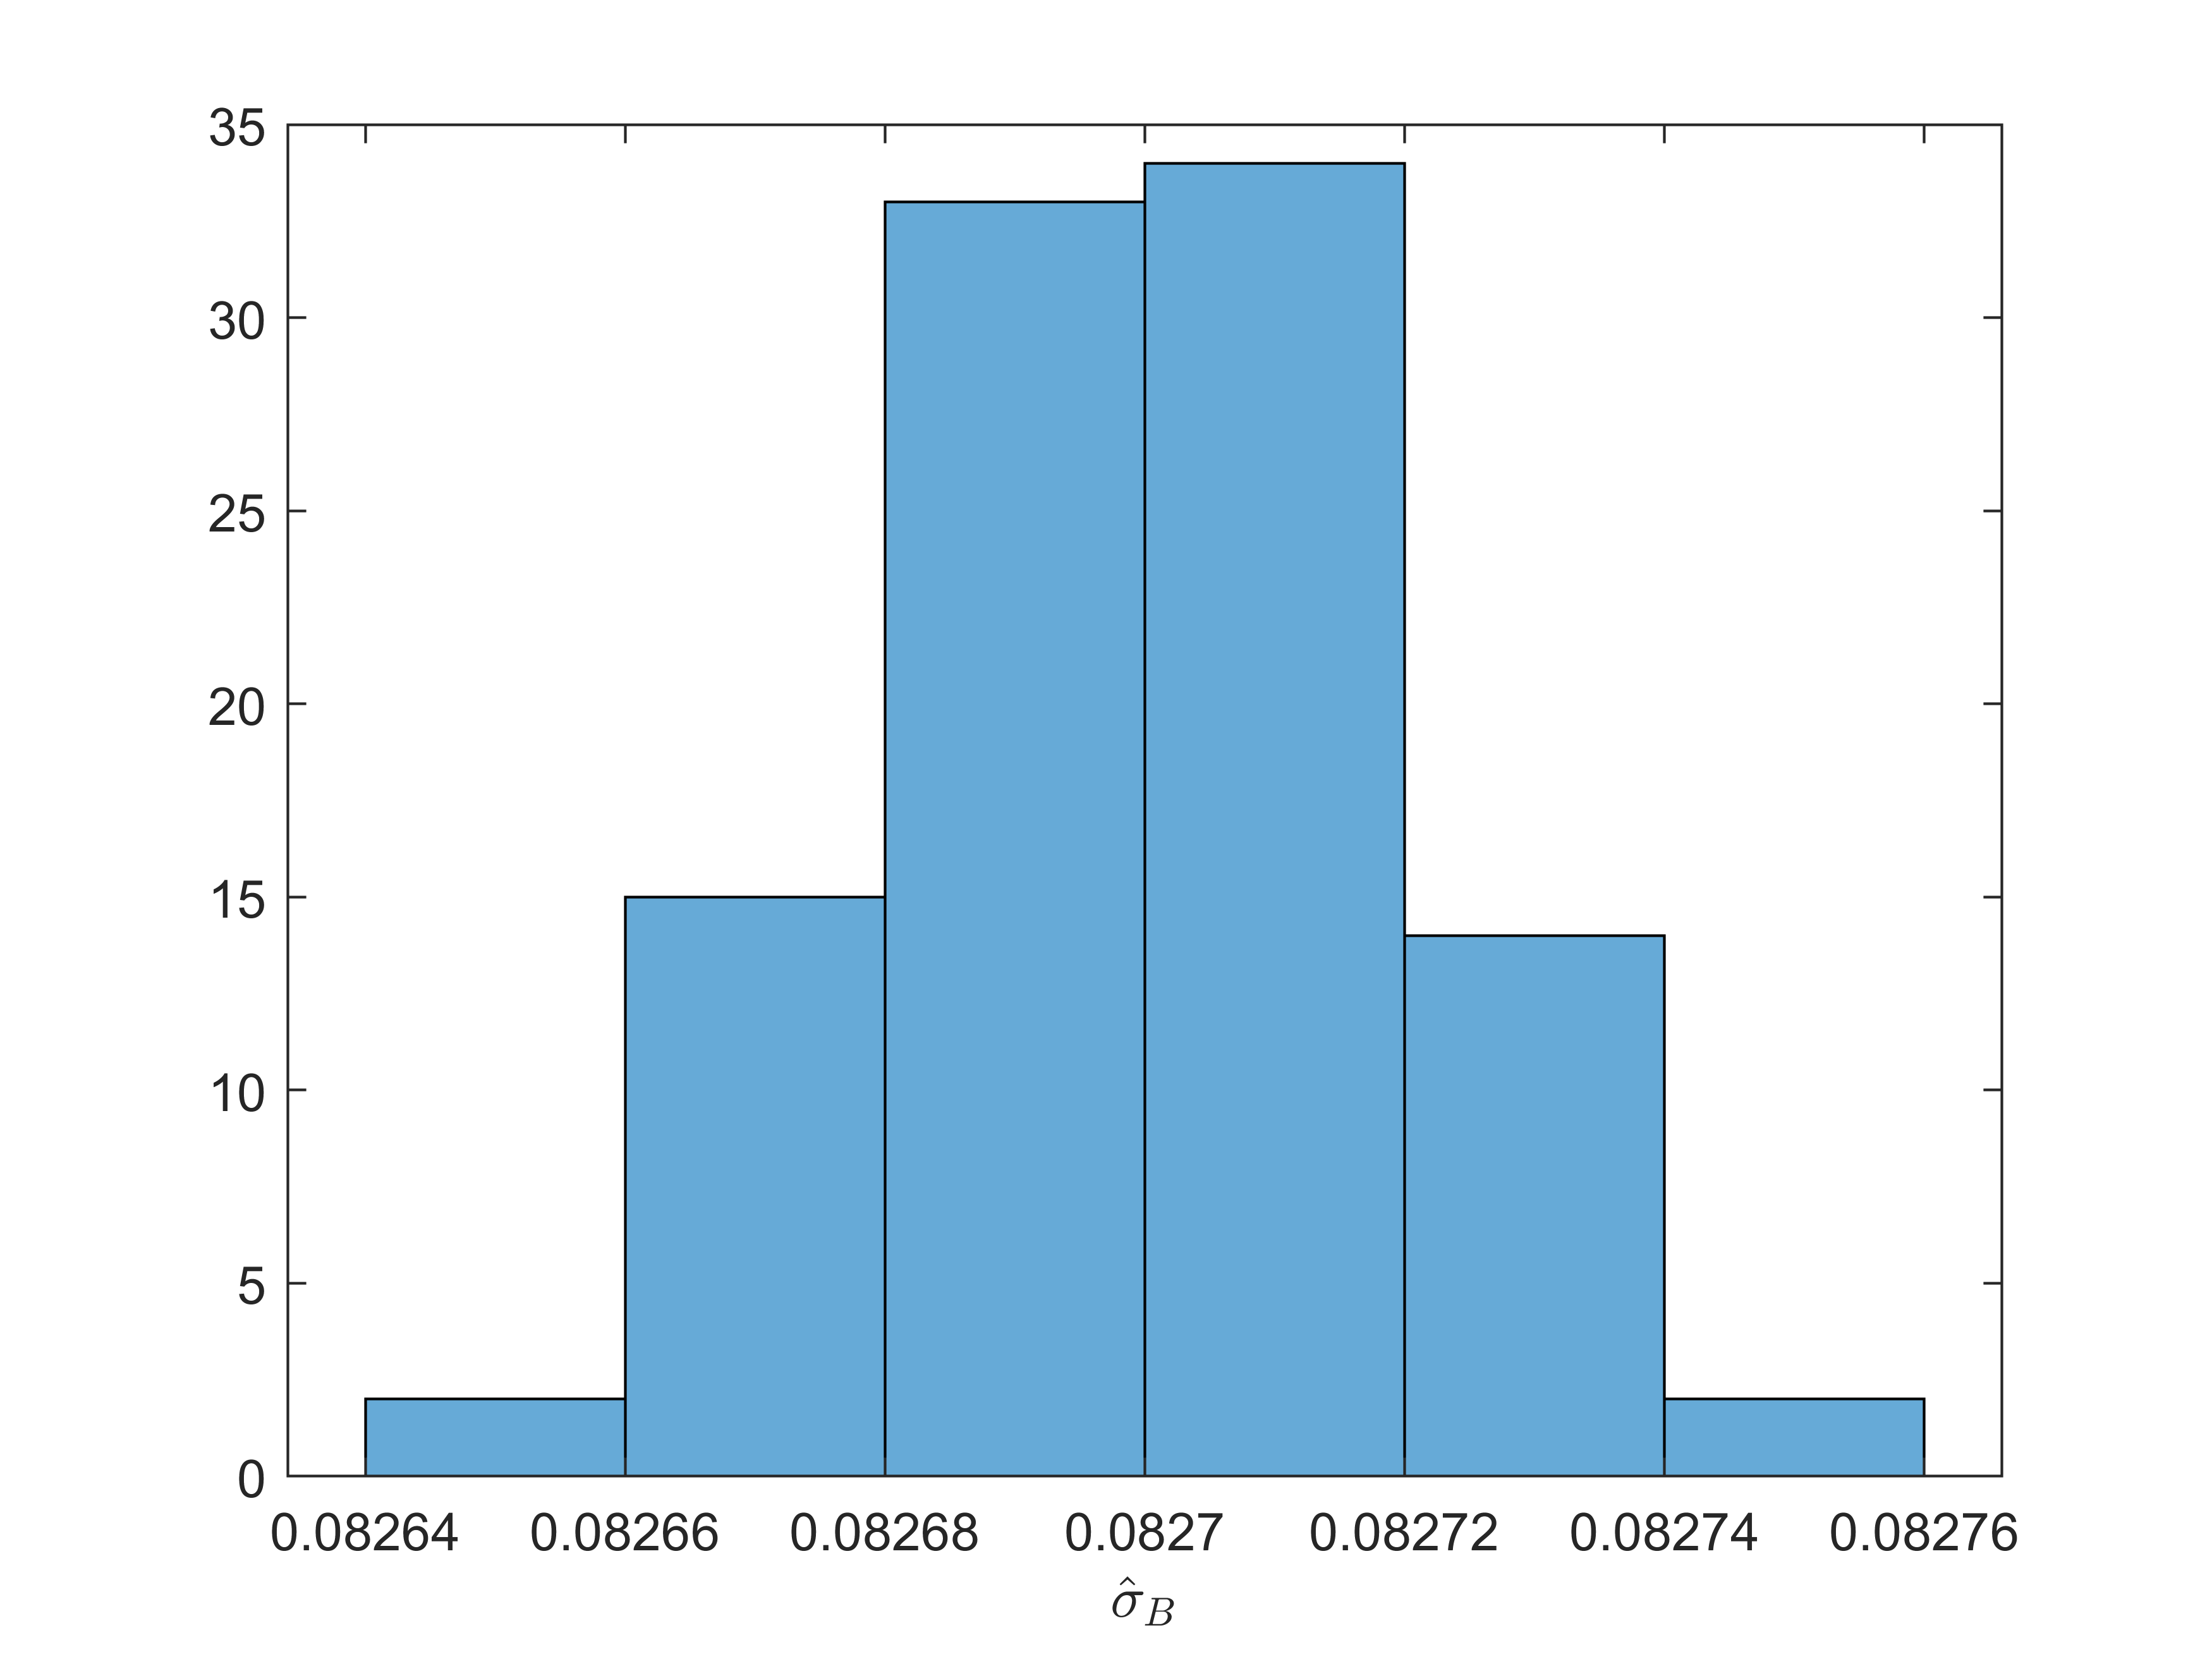
\includegraphics[width=0.47\textwidth]{files/q3,b=10^7.png}
\caption{histogram of $\hat{\sigma}_B$ for $B=10^7,k=100$}
\end{figure}


\subsection*{Question 4}
Theory tells that the standard error of T equates to
\[\sigma(T;F)=\frac{1}{\sqrt{n-3}}\]
In our case, $n=120$. So $\sigma(T;F)=\frac{1}{\sqrt{117}}\approx0.09245$.\\
The null hypothesis $h_0$ is the Verbal and Performance IQ scores are bivariate normal;\\
the alternative hypothesis $h_1$ is IQ scores are not bivariate normal.\\
To reject the hypothesis, we need to show that $\sigma(T;F)=0.09245$ is outside of the confidence interval of $\sigma(T;\hat{F})$.\\
In question 3, we found out that $\sigma(T;\hat{F})=0.0827$. And even with the loosest estimate where we used $B=10^3$ and $k=10^3$, we note the $1\%$ and $99\%$ percentile of the distribution of $\hat{\sigma}_B$ are $0.07860$ and $0.08673$ respectively.\\
$\sigma(T;F)=0.09245\notin[0.07860,0.08673]$, therefore our analysis provides evidence to reject the hypothesis that the Verbal and Performance IQ data are bivariate normal.\\
However, we do need more data to further examine this hypothesis as 120 people is quite a small sample and we have no information on how the data points are collected or if there exists any bias in the selection of the people taking the test.\\

\section*{2 Uniform Data}
Let $\mathbf{X}=(X_1,X_2,\dots,X_n)$ be a sample of real-valued random variables. Suppose the distribution of the statistic \[T(X)=max\{X_1,\dots,X_n\}\] is of interest.
\subsection*{Question 5}
We shall first determine the distribution of $T(Y)$ where $Y$ is an IID sample of size n drawn form the empirical distribution $\hat{F}$. 
\begin{flalign*}
\mathds{P}(T(\bm{Y})\leq t) &= \mathds{P}(max\{Y_1,\dots,Y_n\} \leq t)&\\
&= \mathds{P}(Y_1,\dots,Y_n\leq t)\\
&= \prod_{i=1}^n \mathds{P}(Y_i\leq t)\\
&= \prod_{i=1}^n \sum_{j=1}^n \mathds{P}(Y_i=X_j)\mathds{P}(X_j\leq t)\\
&= \prod_{i=1}^n \sum_{j=1}^n \frac{1}{n}\mathds{P}(X_i\leq t) \qquad\qquad \text{(Since $X_j$ are IID, and $\mathds{P}(Y_i=X_j)=\frac{1}{n}$)}\\
&= \prod_{i=1}^n \mathds{P}(X_i\leq t)\\
&= \mathds{P}(X_1, \dots, X_n \leq t)\\
&= \mathds{P}(T(\bm{X})\leq t)
\end{flalign*}
Therefore, $T(\bm{X})$ and $T(\bm{Y})$ have the same distribution under $F$ and $\hat{F}$ respectively.\\
Hence, \[\sigma(T;\hat{F}) = \sqrt{Var_{\hat{F}}(T(\bm{Y}))}=\sqrt{Var_F(T(\bm{X}))}=\underline{\sigma(T;F)}\]

\bigskip
\subsection*{Question 6}
Suppose the sample $\mathbf{X}$ comes from the unifrom distribution on $[0,\theta]$ for some $\theta>0$, we try to find $\sigma(T;F)$.\\
We first find the cumulative distribution function of $T(X)$.
\begin{flalign*}
\mathds{P}(T\leq x)&=\mathds{P}(X_1\leq x,X_2\leq x, \dots,X_n\leq x)&\\
&=\prod_{i=1}^n \mathds{P}(X_i \leq x)\qquad\qquad\text{(since $X_i$ are iid)}\\
&= \left
\{\begin{array}{lr}
0, & \text{for } x<0\\
(\frac{x}{\theta})^n, & \text{for } 0\leq x\leq \theta\\
1, & \text{for } x>1
\end{array}
\right.\\
\intertext{Hence, the probability density function is \[f_T(x)=\frac{nx^{n-1}}{\theta^n}\]}\\
\mathds{E}[T^2]&= \int^{\theta}_0 x^2 \frac{nx^{n-1}}{\theta^n} dx\\
&= [\frac{n}{n+2}\frac{x^{n+2}}{\theta^n}]_0^{\theta}\quad =\frac{n}{n+2}\theta^2\\
\mathds{E}[T]&= \int^{\theta}_0 x\frac{nx^{n-1}}{\theta^n} dx\\
&= [\frac{n}{n+1}\frac{x^{n+1}}{\theta^n}]^{\theta}_0 \quad =\frac{n}{n+1}\theta
\end{flalign*}
\begin{flalign*}
Var_F[T(X)] &= \mathds{E}[T^2] - \mathds{E}[T]^2&\\
&=\frac{n(n+1)^2-n^2(n+2)}{(n+2)(n+1)^2}\theta^2\\
&=\frac{n\theta^2}{(n+2)(n+1)^2}\\
\intertext{This implies that,}
\sigma(T;F)&=\sqrt{Var_F[T(X)]}\qquad = \underline{\sqrt{\frac{n}{n+2}}\frac{\theta}{n+1}}
\end{flalign*}

\bigskip
\subsection*{Question 7}
We first generate a sample $\mathbf{X}$ with $\theta = 5$ and $n = 100$, and then calculate $\hat{\sigma}_B$ to estimate $\sigma(T;\hat{F})$.
The code used is attached in the programs section under the title \emph{'iii) q7.m'}.\\
From question 5 and 6, we know $\sigma(T;F)=\sqrt{\frac{100\times 25}{102 \times 101^2}}=0.049012$ (6d.p.), and using the code we found that $\sigma(T;\hat{F})=0.025941$ with $B=10^6$, which is almost half the value for \\
We repeat for increasing $n$, i.e. when $n=10^3,10^4,10^5$, and the results are shown in the table below.\\
\begin{center}
    \begin{tabular}{|c|c|c|}
    \hline
        n & $\sigma(T;F)$ & $\hat{\sigma}_B$ \\
        \hline
        $100$ & $0.049017$ & $0.025941$\\
        \hline
        $10^3$ & $0.004990$ & $0.008409$\\
        \hline
        $10^4$ & $0.0004999$ & $0.0005740$\\
        \hline
        $10^5$ & $0.000049999$ & $0.000018592$\\
        \hline
    \end{tabular}
\end{center}
This shows us that for the range of $n$ we've tested, the bootstrap method performed very poorly to estimate $\sigma(T;F)$, as $\hat{\sigma}_B$ is often much smaller or larger than $\sigma(T;F)$ and this doesn't improve as $n$ increases.\\
The reason why the bootstrap method fails in this case is because we fail to approximate the distribution of $T(\mathbf{X})$ with the distribution of $T(\mathbf{Y})$ where $Y$ is the resampling of the same sample $\mathbf{X_1}$.\\
We show this by considering the distribution of $n(\theta-T(\mathbf{X}))$. We get:
\begin{flalign*}
\mathds{P}(n(\theta-T(\mathbf{X}))\leq x)&=\mathds{P}(T(\mathbf{X})>\theta-\frac{x}{n}) &\\
&= 1-\mathds{P}(T(\mathbf{X})\leq (\theta-\frac{x}{n}))\\
&=1-(\frac{\theta-\frac{x}{n}}{\theta})^n\\
&=1-(1-\frac{x}{n\theta})^n\\
&\to 1-e^{\frac{-x}{\theta}} \qquad\text{as $n\to\infty$} \qquad\text{i.e. \underline{$n(\theta-T(\mathbf{X}))\xrightarrow{d}exp(\frac{1}{\theta})$}}
\end{flalign*}
\noindent We can visualise this by generating $M$ samples of $\mathbf{X}$, with $\mathbf{X_m}=(X_{m,1},\dots,X_{m,n})$ and $X_{m,i}\sim U[0,\theta]$ iid. We then plot the histogram of $n(\theta-T(\mathbf{X}))$.
\begin{figure}[H]
\centering
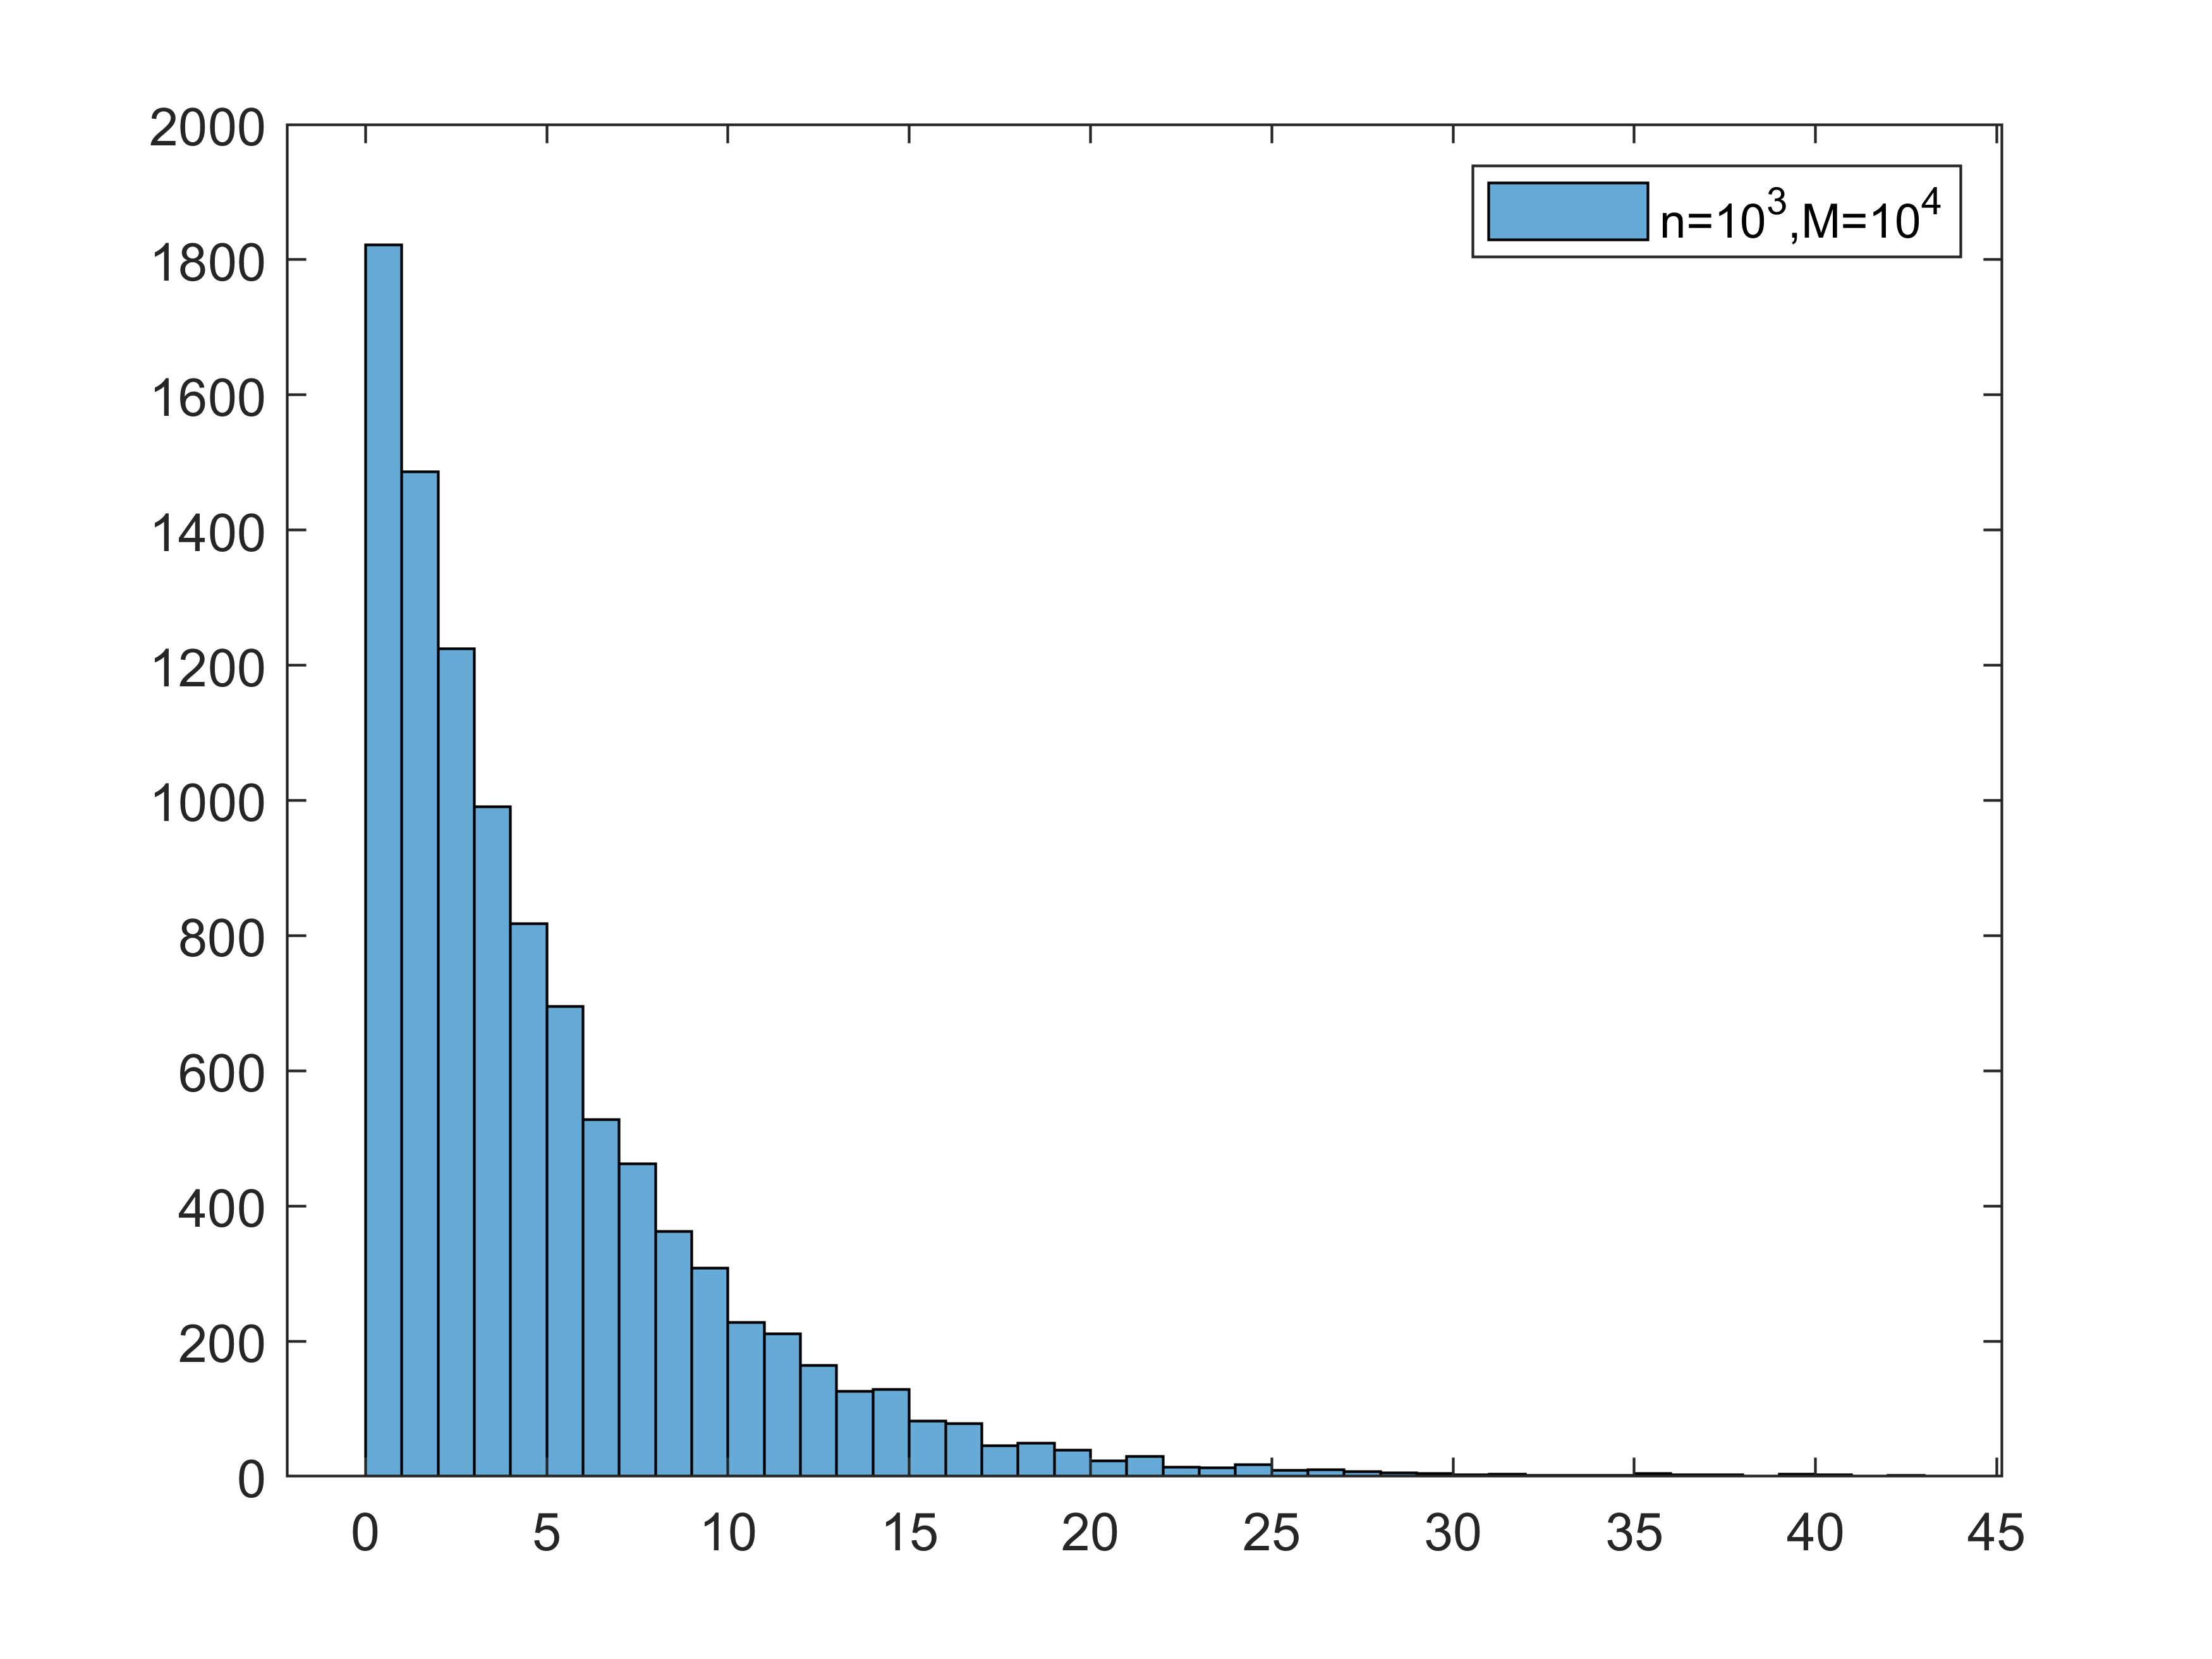
\includegraphics[width=0.5\textwidth]{files/q7,test.png}
\caption{histogram of $n(\theta-T(\mathbf{X}))$ when $n=10^3,M=10^4$}
\end{figure}
\noindent However, when using the bootstrap method, we obtain $\mathbf{Y}_b$ for all $b$ from the resampling of the same given sample $\mathbf{X_1}$.\\
This is a problem because now $\mathds{P}(T(\mathbf{Y_b})=T(\mathbf{X_1}))=1-(1-\frac{1}{n})^n$. And as $n\to\infty$, this tends to $1-e^{-1}$.\\
So for any $\mathbf{X_1}$ we generate on any value of $\theta$, the bootstrap distribution will always contain a point mass at $T(\mathbf{X_1})$, which is the maximum of $\mathbf{X_1}$. This means $T(\mathbf{Y})$ will have a very different distribution to $T(\mathbf{X})$. This is true as the limiting distribution of $n(\theta-T(\mathbf{X}))$ is continuous and $n(T(\mathbf{X})-T(\mathbf{Y}))$ is not.\\
We can again do a simulation to visualise this. Figure 10 below is the distribution of $n(\theta-T(\mathbf{Y}))$ generated using the bootstrap method. We can clearly see that it has a totally different distribution compared to the original one (figure 9).\\
\begin{figure}[H]
\centering
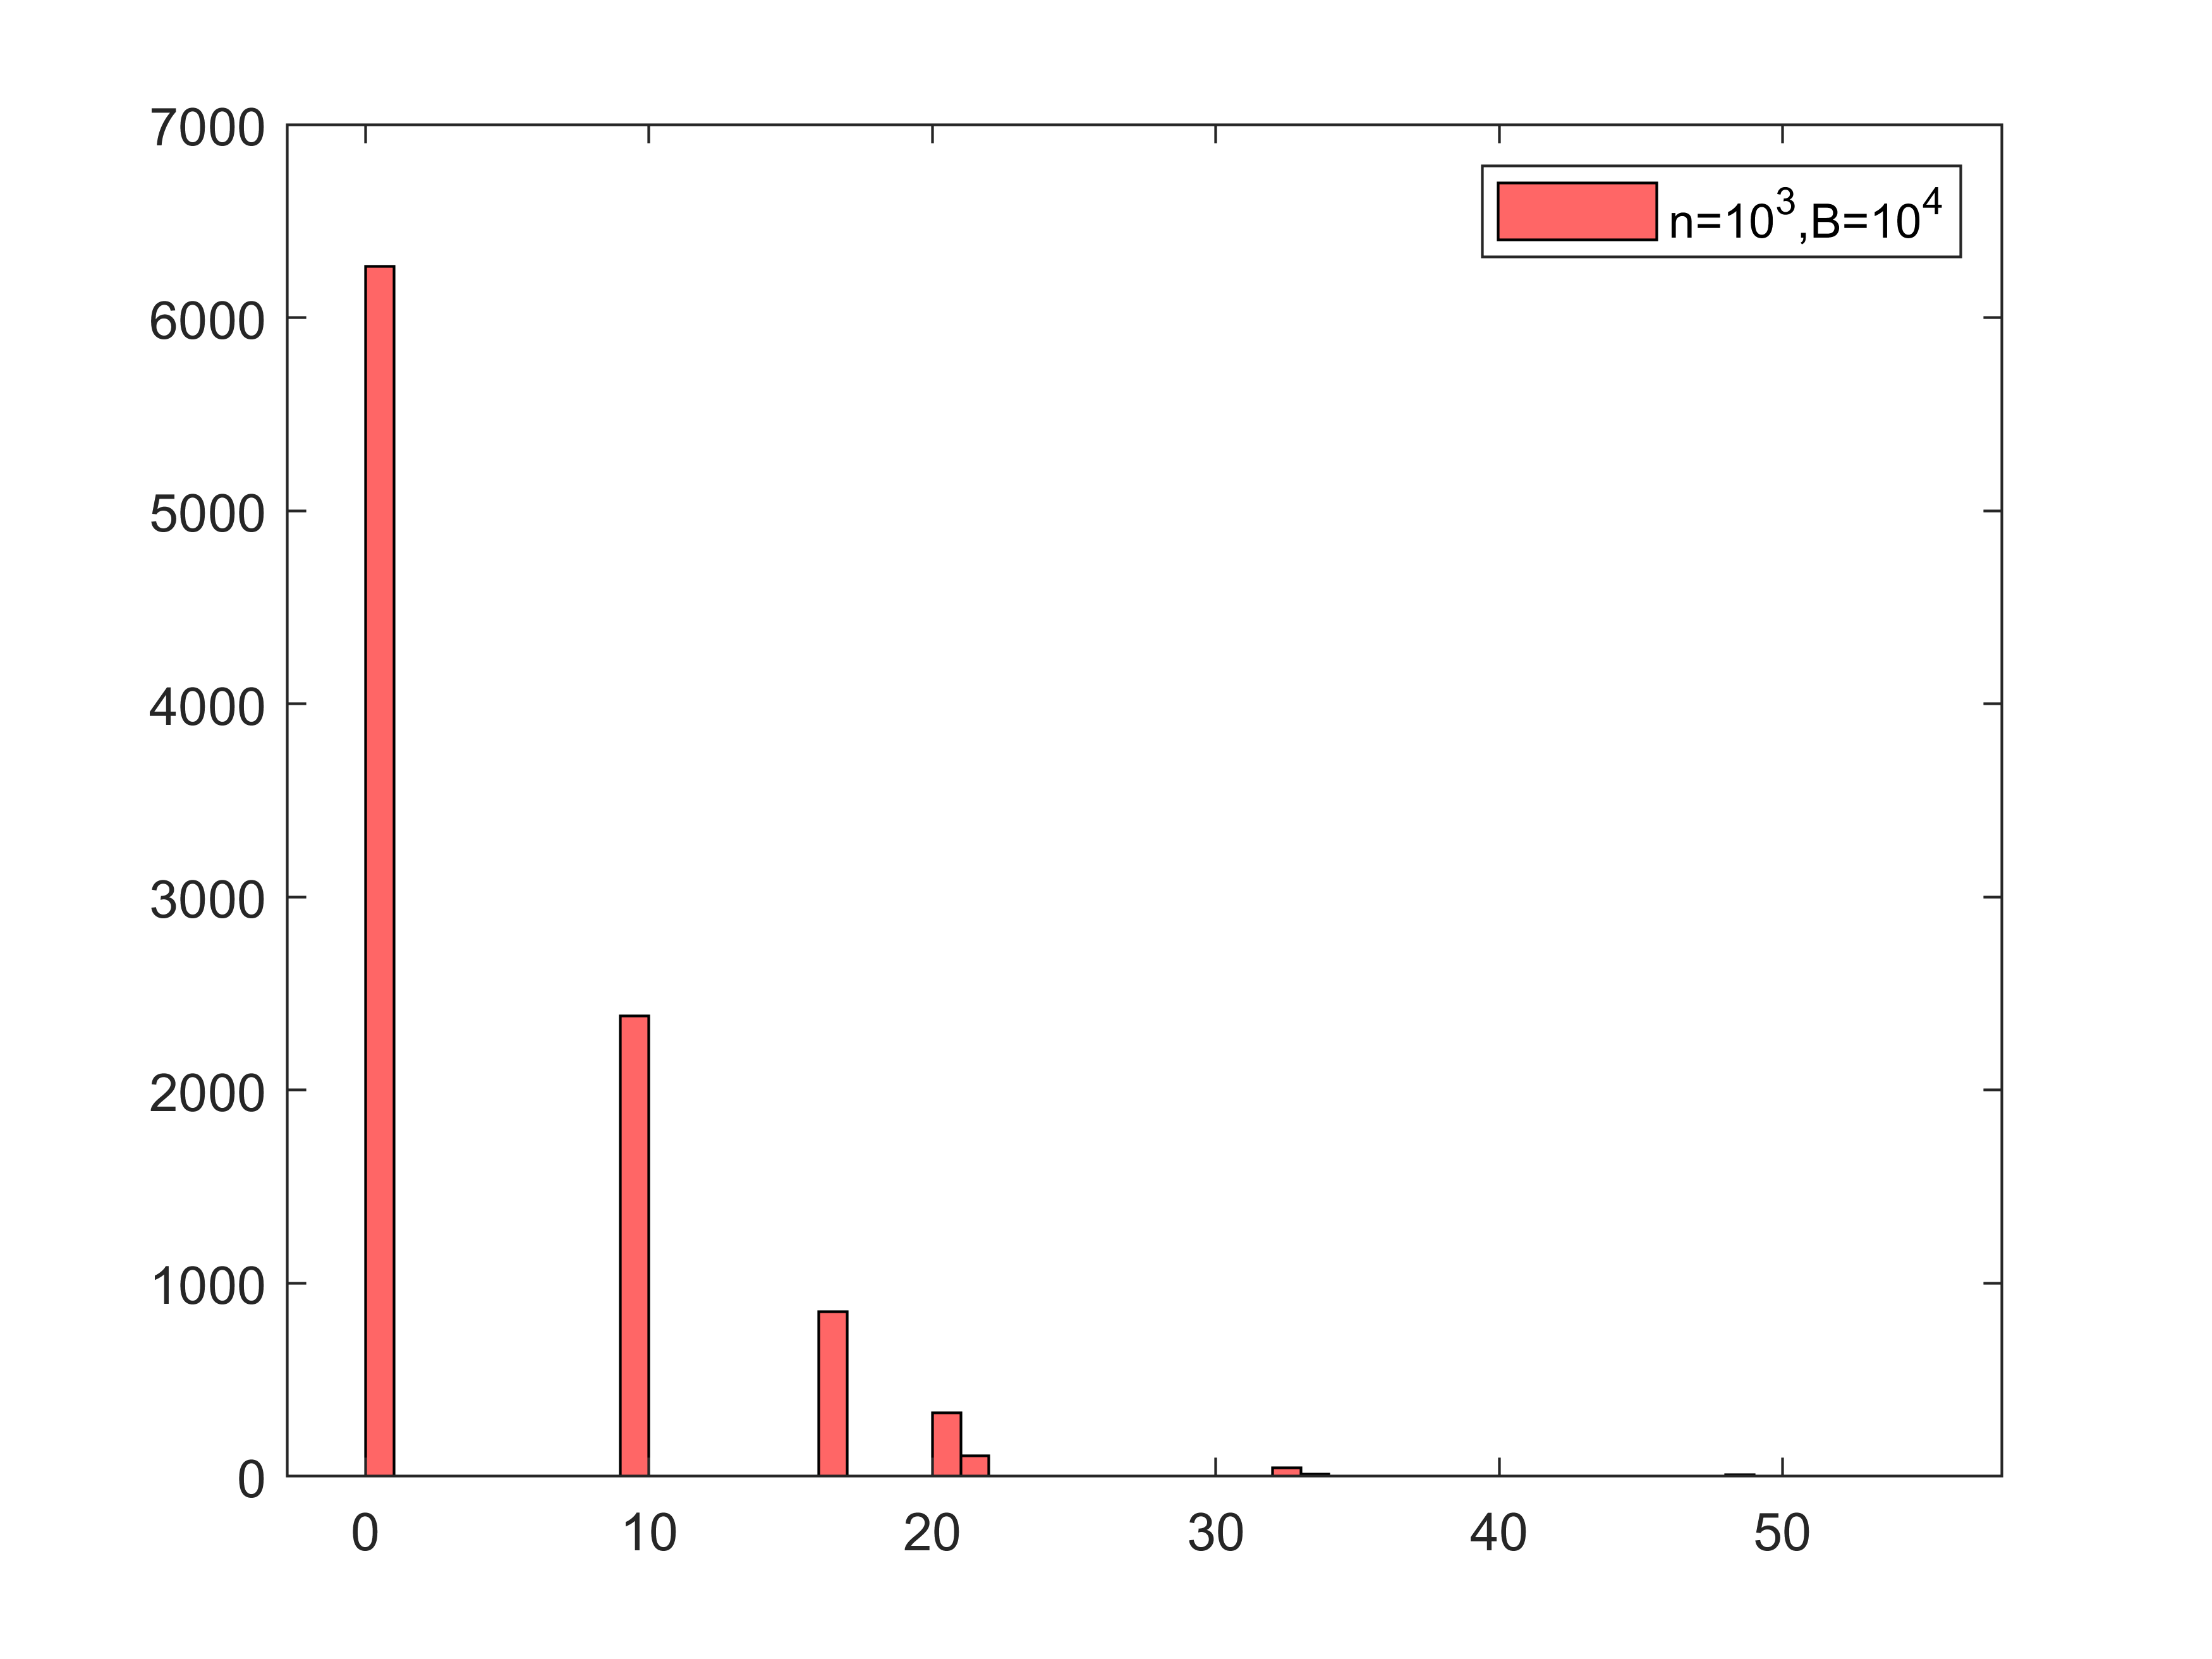
\includegraphics[width=0.5\textwidth]{files/q7,bootstrap.png}
\caption{histogram of $n(T(\mathbf{X})-T(\mathbf{Y}))$ using bootstrap method when $n=10^3,B=10^4$}
\end{figure}
\noindent Therefore, we can't use the bootstrap method to estimate $\sigma(T;F)$ as our estimation is based on the assumption that the distribution of $T(\mathbf{Y})-T(\mathbf{X})$ and $T(\mathbf{X})-\theta$ are nearly the same for $n$ sufficiently large. However, as we can see from the graphs and the calculation above, this is not the case in this example.\\\\\\
\noindent
In fact, the $\hat{\sigma}_B$ values will vary massively from trial to trial when $n$ is small, because they are heavily dependent on the sample $\mathbf{X_1}$ we draw to base our resampling $\mathbf{Y}$ on. And as $n$ increases, the estimation does not become any more accurate because of the different asymptotic underlying distribution.\\\\
\noindent The fact that we have different distributions does not contradict what we found in question 5, because in question 5, we are resampling the random variable $\mathbf{X}$ to generate $\mathbf{Y}$ which should be considered as a random variable, and $T(\mathbf{Y})$ does have the same distribution as $T(\mathbf{X})$.\\
Whereas here, we are generating $B$ samples of $\mathbf{Y}$ from the \textbf{same} observed data sample $\mathbf{X_1}$, \textbf{which is held fixed} and the variability in $\mathbf{Y}$ comes from the resampling only.\\

\noindent The code I used to plot figure 9 and 10 is in the programs section as \emph{'iv) q7\textunderscore distribution.m'}\\

\newpage
\section*{Programs}
\bigskip
\subsection*{i) q2\textunderscore bootstrap.m}
\lstdefinestyle{myCustomMatlabStyle}{
  language=Matlab,
  stepnumber=1,
  numbersep=10pt,
  tabsize=4,
  showspaces=false,
  showstringspaces=false
}
\lstset{basicstyle=\footnotesize,style=myCustomMatlabStyle}
\begin{lstlisting}
data = readtable("II-10-3-2020.csv");
data = table2array(data);
B = 10^6;    % number of bootstrap samples
n = height(data);
t = zeros(B,1); % stores values of t(Y_b)

for i = 1:B
    rnum = randi([1,n],1,n);  % select n random samples from X
    temp_y = zeros(n,1);  
    temp_z = zeros(n,1);
    % assign corresponding y and z values to the bootstrap samples
    for j=1:n
        temp_y(j) = data(rnum(j),1);
        temp_z(j) = data(rnum(j),2);
    end
    % calculate the mean of Y and Z
    y_mean = sum(temp_y)/n;
    z_mean = sum(temp_z)/n;
    % calculate r(X) where X=(Y,Z)
    r_num = sum((temp_y-y_mean).*(temp_z-z_mean));
    r_denom = sqrt(sum((temp_y-y_mean).^2)*sum((temp_z-z_mean).^2));
    r = r_num/r_denom;
    t(i) = log((1+r)/(1-r))/2;      % T(Y_b)
end

h1 = histogram(t);
disp(h1)
xlabel('T(Y)')
ylabel('frequency')
figure()
% we normalise the histogram as a pdf
h2 = histogram(t,'Normalization','pdf');
% descriptive stats (mean, variance, minimum and maximum)
disp([mean(t), var(t),min(t),max(t)])
disp(h2)
xlabel('T(Y)')
ylabel('probability density')

\end{lstlisting}
\subsection*{ii) q3.m}
\lstdefinestyle{myCustomMatlabStyle}{
  language=Matlab,
  stepnumber=1,
  numbersep=10pt,
  tabsize=4,
  showspaces=false,
  showstringspaces=false
}
\lstset{basicstyle=\footnotesize,style=myCustomMatlabStyle}
\begin{lstlisting}
format long
data = readtable("II-10-3-2020.csv");
data = table2array(data);
n = height(data);
k = 100;       % number of repeated experiments
B = 10^7;      % number of bootstrap samples
sigma_B = zeros(k,1);   % time we repeat the algorithm
t = zeros(B,1);     % stores values of t(Y_b)
for l = 1:k
    for i = 1:B
        rnum = randi([1,n],1,n);  % select n random samples from X
        temp_y = zeros(n,1);  
        temp_z = zeros(n,1);
        % assign corresponding y and z values
        for j=1:n
            temp_y(j) = data(rnum(j),1);
            temp_z(j) = data(rnum(j),2);
        end
        % calculate the mean of Y and Z
        y_mean = sum(temp_y)/n;
        z_mean = sum(temp_z)/n;
        % calculate r(X) where X=(Y,Z)
        r_num = sum((temp_y-y_mean).*(temp_z-z_mean));
        r_denom = sqrt(sum((temp_y-y_mean).^2)*sum((temp_z-z_mean).^2));
        r = r_num/r_denom;
        t(i) = log((1+r)/(1-r))/2;      % T(Y_b)
    end
    % to calculate sigma_B
    t_mean = sum(t)/B;
    sigma_B(l) = (sqrt(sum((t-t_mean).^2)./(B-1)));
end
% to plot the histograms
h=histogram(sigma_B,'NumBins',20);
xlabel('$\hat{\sigma}_B$','Interpreter','latex')
legend()
disp(h)

\end{lstlisting}
\subsection*{iii) q7.m}
\lstdefinestyle{myCustomMatlabStyle}{
  language=Matlab,
  stepnumber=1,
  numbersep=10pt,
  tabsize=4,
  showspaces=false,
  showstringspaces=false
}
\lstset{basicstyle=\footnotesize,style=myCustomMatlabStyle}
\begin{lstlisting}
format long
B = 10^6;    % number of bootstrap samples
T = zeros(B,1);     % stores values of T(Y)
theta = 5;      % upper bound for the distribution
N = [10^3,10^4];        % number of data points
sigma_hat = zeros(numel(N),1);
for n = 1:numel(N)
% generating n iid data unif distribution on [0,theta]
    X = theta*rand(N(n),1);
    for i = 1:B
        rnum = randi([1,N(n)],1,N(n));  % select n random indices in range(1,n)
        temp_y = zeros(N(n),1);       % current bootstrap sample
        % assign current bootstrap sample
        for j = 1:N(n)
           temp_y(j) = X(rnum(j)); 
        end
        % find T
        T(i) = max(temp_y);
    end    
    % caching T_mean
    T_mean = sum(T)/B;
    % calculate sigma(T;F_hat)
    sigma_hat(n) = (sqrt(sum((T-T_mean).^2)./(B-1)));
end
disp(sigma_hat)



\end{lstlisting}
\subsection*{iv) q7\textunderscore distribution.m}
format long
\lstdefinestyle{myCustomMatlabStyle}{
  language=Matlab,
  stepnumber=1,
  numbersep=10pt,
  tabsize=4,
  showspaces=false,
  showstringspaces=false
}
\lstset{basicstyle=\footnotesize,style=myCustomMatlabStyle}
\begin{lstlisting}
% plotting histogram of n(theta-T)
theta = 5;      % upper bound for the distribution
n=10^3;        % number of data points
M = 10^4;
T = zeros(M,1);
stat = zeros(M,1);
for i = 1:M
    % generating n iid data unif distribution on [0,theta]
    X = theta*rand(n,1);
    T(i) = max(X);
    stat(i) = n*(theta-T(i));
end
histogram(stat)
legend('n=10^3,M=10^4')

% plotting histogram for bootstrap n(theta-T)
B = 10^4;    % number of bootstrap samples
X_bootstrap = theta*rand(n,1);
T_bootstrap = zeros(B,1);
stat_bootstrap = zeros(B,1);
for k = 1:B
    rnum = randi([1,n],1,n);  % select n random indices in range(1,n)
    temp_y = zeros(n,1);       % current bootstrap sample
    % assign current bootstrap sample
    for j = 1:n
       temp_y(j) = X_bootstrap(rnum(j)); 
    end
    % find T
    T_bootstrap(k) = max(temp_y);
    stat_bootstrap(k) = n*(max(X_bootstrap)-T_bootstrap(k));
end
figure()
histogram(stat_bootstrap)
legend('n=10^3,B=10^4')

\end{lstlisting}
\end{document}